%# -*- coding: utf-8 -*-
% !TeX encoding = UTF-8 Unicode
% !TeX spellcheck = en_US
% !TeX TS-program = xelatex
%~ \XeTeXinputencoding "UTF-8"
% vim:ts=4:sw=4
%
% 以上设定默认使用 XeLaTex 编译,并指定 Unicode 编码,供 TeXShop 自动识别


\newcommand{\doctitle}{SmarShow User Manual}
\newcommand{\docauthor}{Yunhui Fu}
\newcommand{\dockeywords}{}
\newcommand{\docsubject}{}


\documentclass[a4paper,10pt]{article}

\title{\doctitle}
\author{\docauthor}
\date{}

\usepackage{ifthen}
\usepackage{ifpdf}
\usepackage{ifxetex}
\usepackage{ifluatex}


\usepackage{url}
\usepackage{array}

\usepackage{courier}
\usepackage{listings} % list the source code

\ifxetex % xelatex
\else
    %The cmap package is intended to make the PDF files generated by pdflatex "searchable and copyable" in acrobat reader and other compliant PDF viewers.
    \usepackage{cmap}%
\fi
% ============================================
% Check for PDFLaTeX/LaTeX
% ============================================
\newcommand{\outengine}{xetex}
\newif\ifpdf
\ifx\pdfoutput\undefined
  \pdffalse % we are not running PDFLaTeX
  \ifxetex
    \renewcommand{\outengine}{xetex}
  \else
    \renewcommand{\outengine}{dvipdfmx}
  \fi
\else
  \pdfoutput=1 % we are running PDFLaTeX
  \pdftrue
  \usepackage{thumbpdf}
  \renewcommand{\outengine}{pdftex}
  \pdfcompresslevel=9
\fi
\usepackage[\outengine,
    bookmarksnumbered, %dvipdfmx
    %% unicode, %% 不能有unicode选项,否则bookmark会是乱码
    colorlinks=true,
    citecolor=red,
    urlcolor=blue,        % \href{...}{...} external (URL)
    filecolor=red,      % \href{...} local file
    linkcolor=black, % \ref{...} and \pageref{...}
    breaklinks,
    pdftitle={\doctitle},
    pdfauthor={\docauthor},
    pdfsubject={\docsubject},
    pdfkeywords={\dockeywords},
    pdfproducer={Latex with hyperref},
    pdfcreator={pdflatex},
    %%pdfadjustspacing=1,
    pdfborder=1,
    pdfpagemode=UseNone,
    pagebackref,
    bookmarksopen=true]{hyperref}

% --------------------------------------------
% Load graphicx package with pdf if needed 
% --------------------------------------------
\ifxetex    % xelatex
    \usepackage{graphicx}
\else
    \ifpdf
        \usepackage[pdftex]{graphicx}
        \pdfcompresslevel=9
    \else
        \usepackage{graphicx} % \usepackage[dvipdfm]{graphicx}
    \fi
\fi

%% \DeclareGraphicsRule{.jpg}{eps}{.bb}{}
%% \DeclareGraphicsRule{.png}{eps}{.bb}{}
\graphicspath{{./} {figures/}}
\usepackage{flafter} % 防止图形在文字前



\begin{document}

\maketitle
\tableofcontents


\section{Introduction}

SmartShow implemented a digital interface to the vintage Fluke 8050a DMM,
fetches the display data via UART port, and optional connected by WiFi via an ESP8266 module.




\section{Hardware}

\begin{figure}[h!t] \centering
    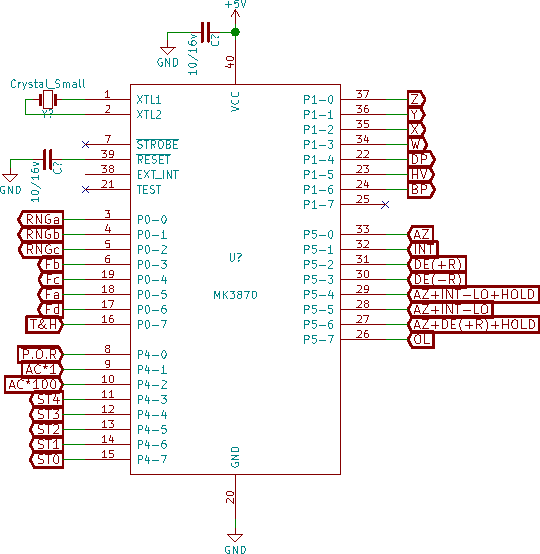
\includegraphics{figures/sch-fluke8050a-u17.pdf}
    \caption{Fluke 8050a DMM U17.} \label{fig:fluke8050a-u17}
\end{figure}

The Arduino UNO or Micro are used as the hardware interface to the MCU of the Fluke 8050a DMM,
an ESP8266 module is used as WiFi UART bridge.


\begin{figure}[h!t] \centering
    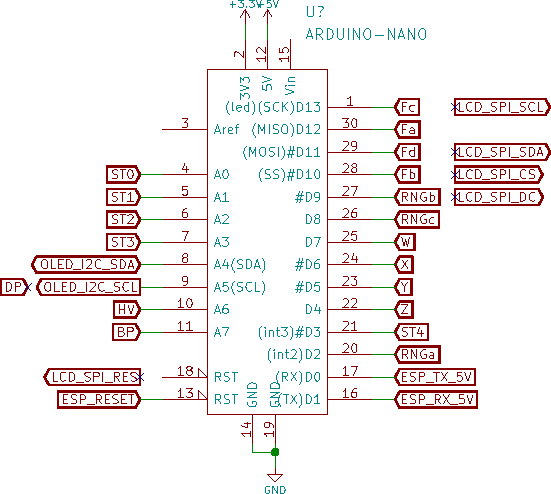
\includegraphics{figures/sch-smartshow-atmega328p.pdf}
    \caption{ATMega328p as headless interface.} \label{fig:smartshow-atmega328p}
\end{figure}

The Arduino UNO is ATMega328p based module and have no enough pin resource to handle both the TTL signal
and an SPI LCD module, so it's only used as headless UART port for outside. While it still have the ability
to drive an I2C OLED display, and an I2C slot is reserved.

\begin{figure}[h!t] \centering
    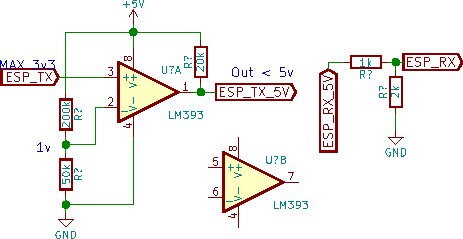
\includegraphics[width=0.8\linewidth]{figures/sch-smartshow-levelshift.pdf}
    \caption{Level shifting works between Arduino UNO and ESP8266.} \label{fig:levelshift}
\end{figure}


The Arduino Micro is ATMega32U4 based module, it can drive a TFT SPI display module.
So it's used to be a replacement of original Fluke 8050a LCD display.

\begin{figure}[h!t] \centering
    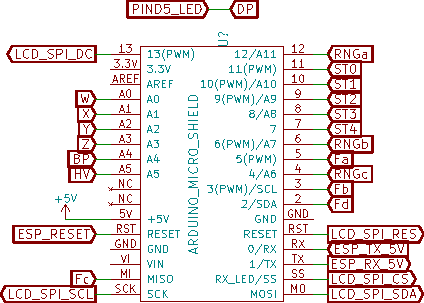
\includegraphics{figures/sch-smartshow-atmega32u4.pdf}
    \caption{ATMega32U4 as display interface.} \label{fig:smartshow-atmega32u4}
\end{figure}

ESP8266 would not start if the TX port is connected directly or via bi-direction level shifting to the RX of Arduino UNO, the solution is to use an LM393 level shifting.

\begin{figure}[h!t] \centering
    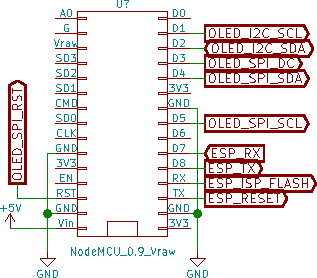
\includegraphics{figures/sch-smartshow-esp8266.pdf}
    \caption{ESP8266 module as WiFi UART bridge. (UART Swap mode)} \label{fig:smartshow-esp8266}
\end{figure}


\begin{figure}[h!t] \centering
    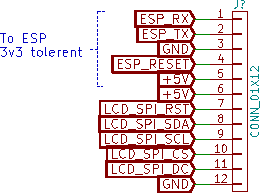
\includegraphics{figures/sch-smartshow-port.pdf}
    \caption{The connector for ESP8266.} \label{fig:smartshow-port}
\end{figure}




\begin{figure}[h!t] \centering
    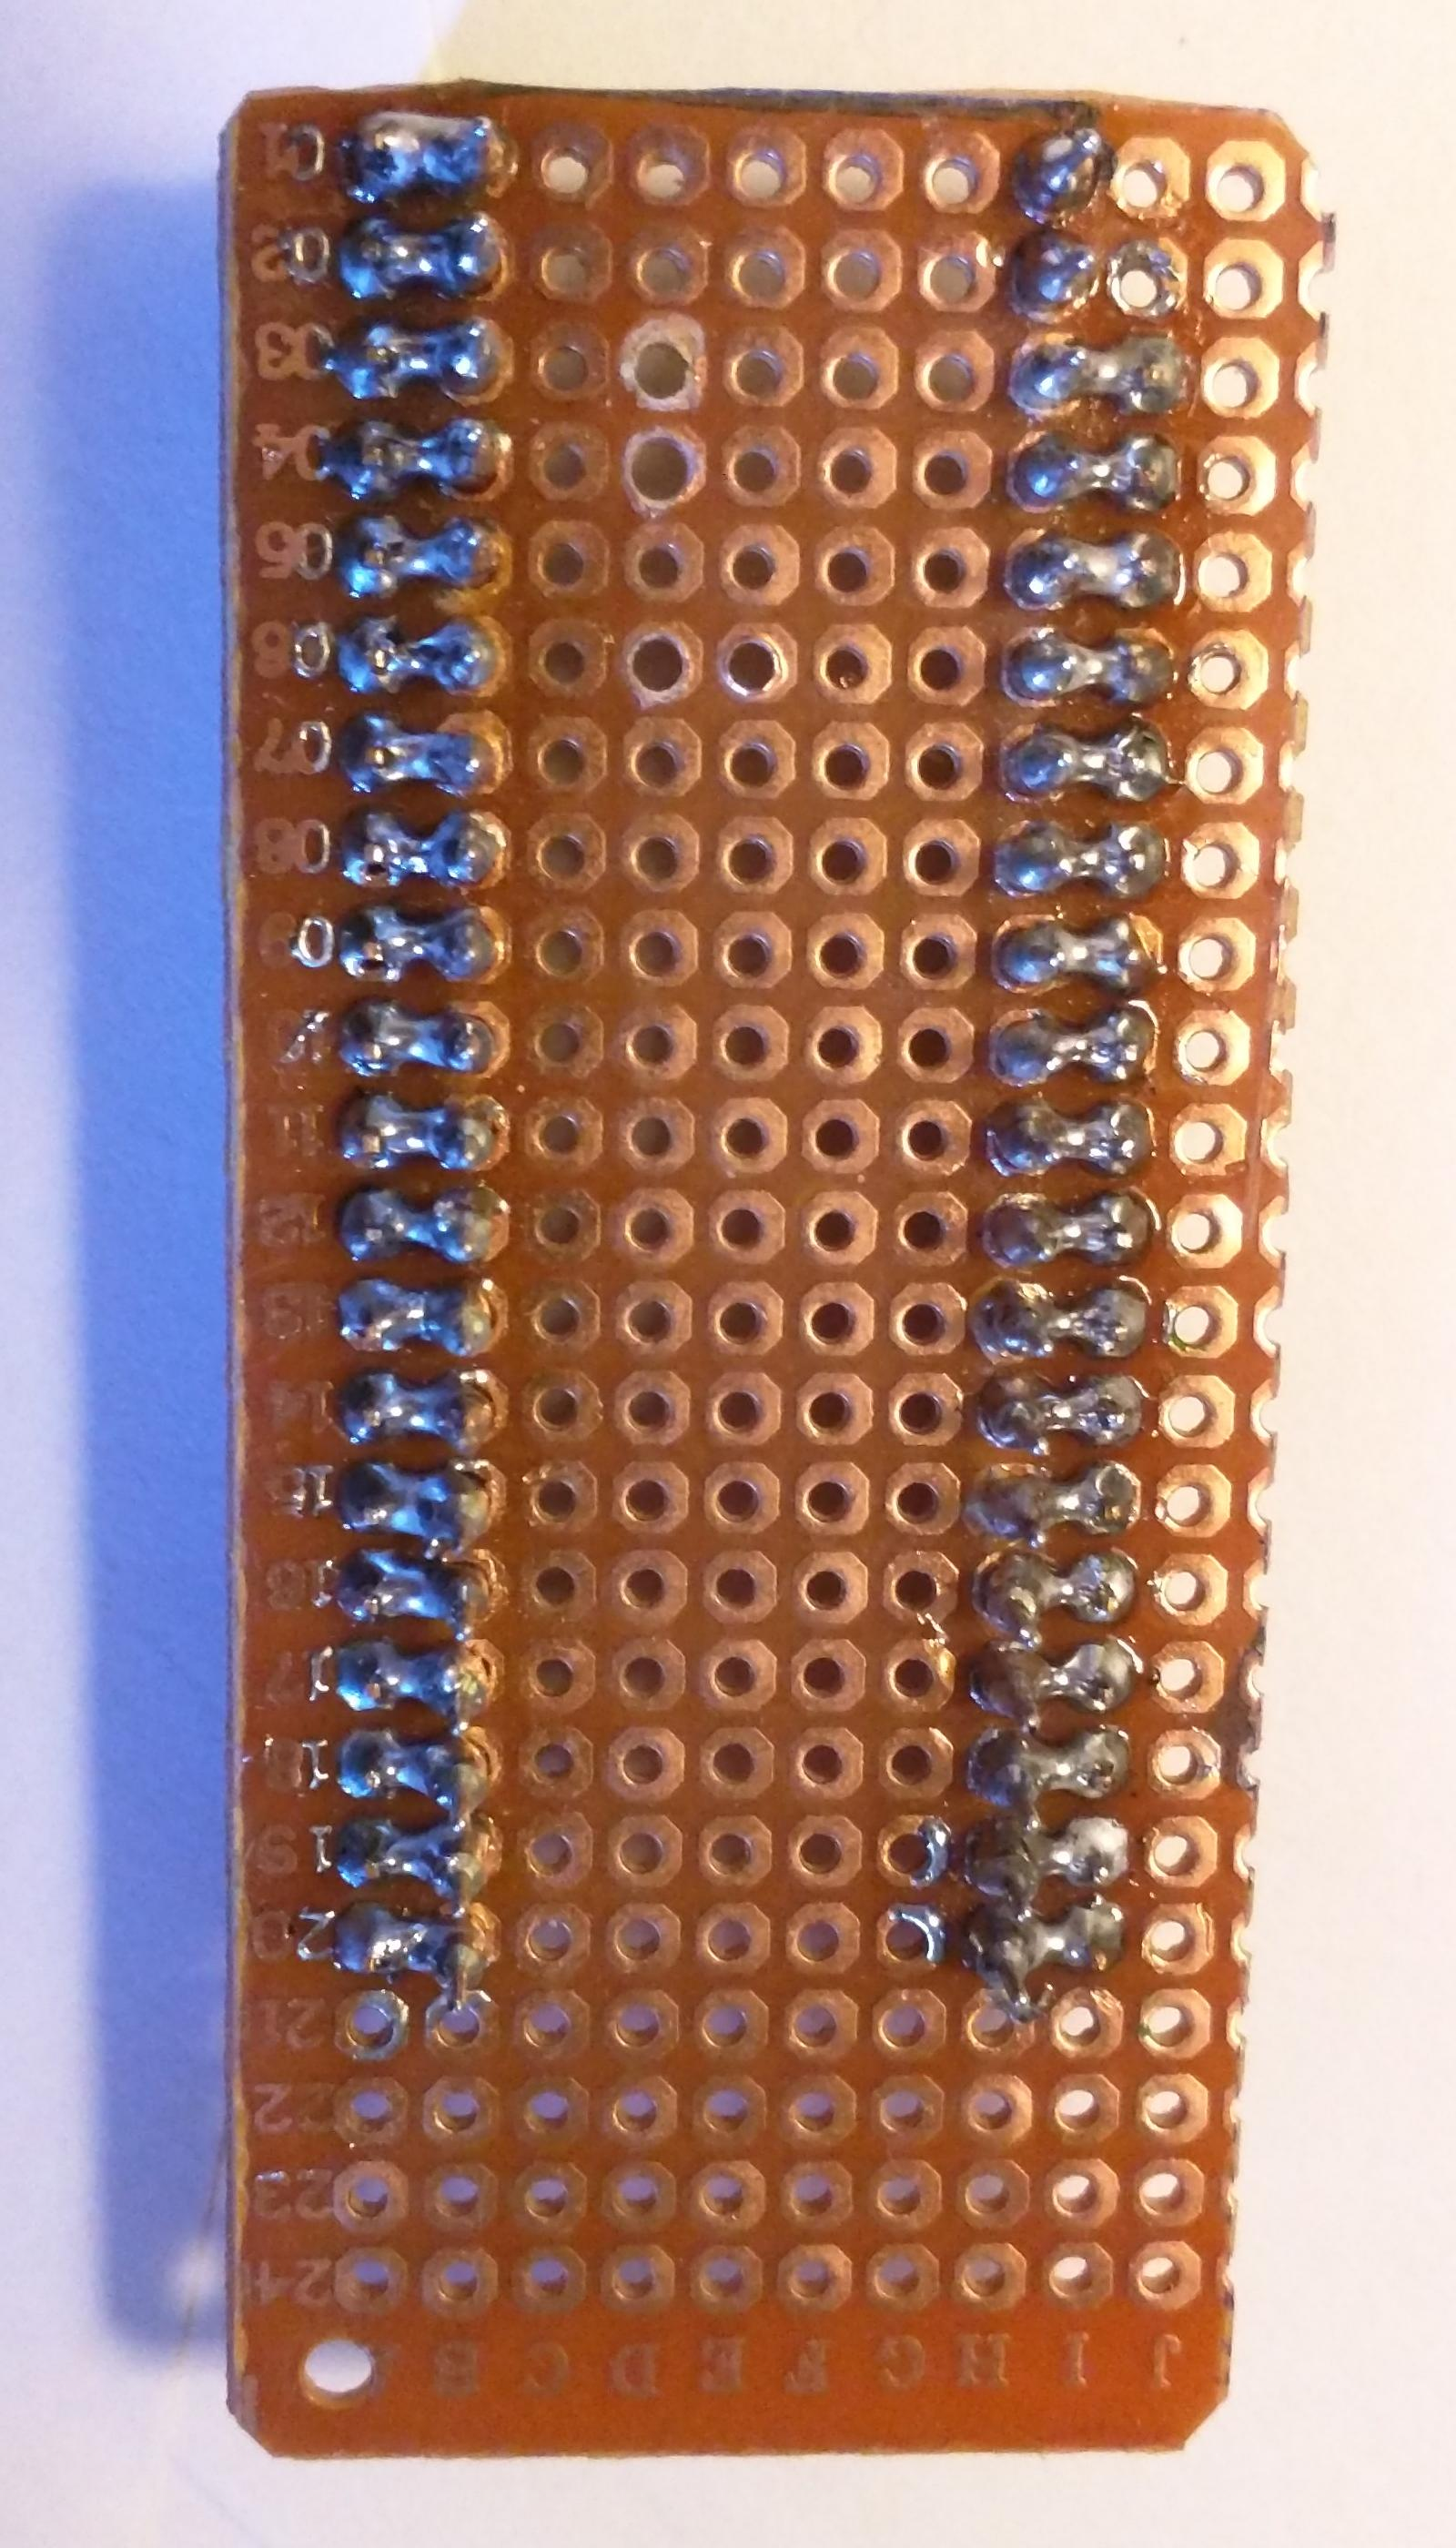
\includegraphics[width=0.30\linewidth]{figures/pic-u17-piggybacked-down.jpg}
    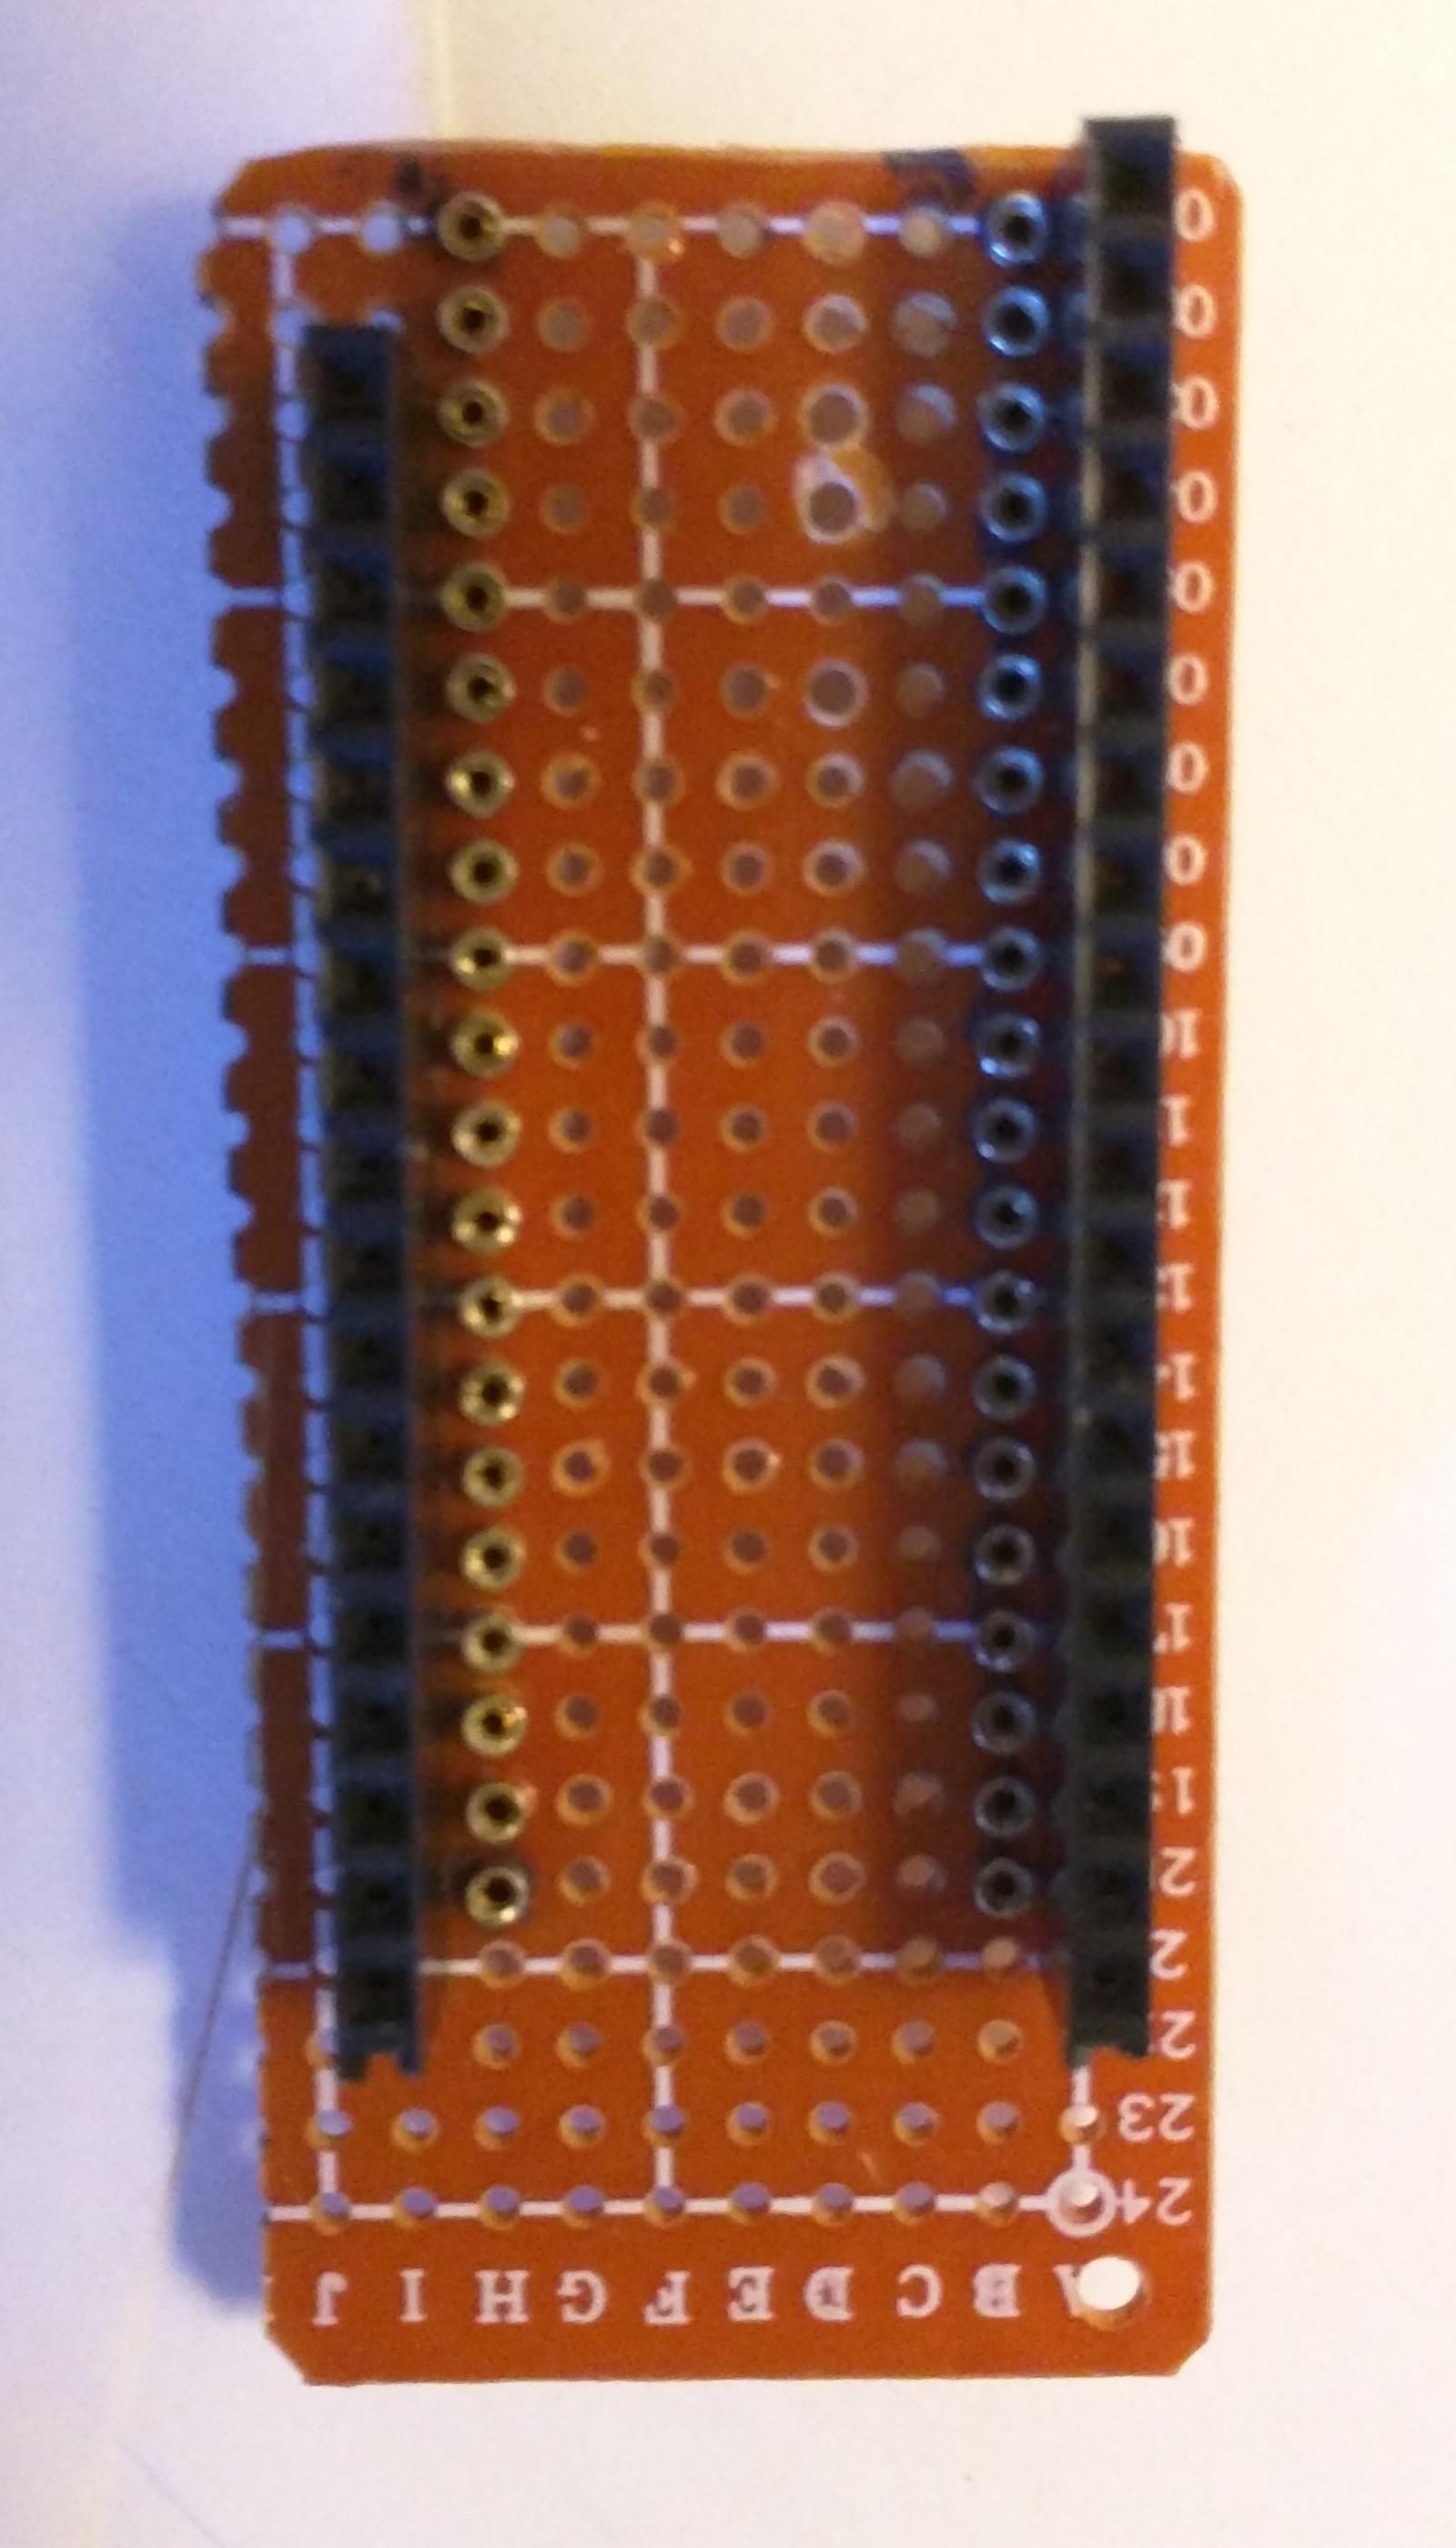
\includegraphics[width=0.30\linewidth]{figures/pic-u17-piggybacked-up.jpg}
    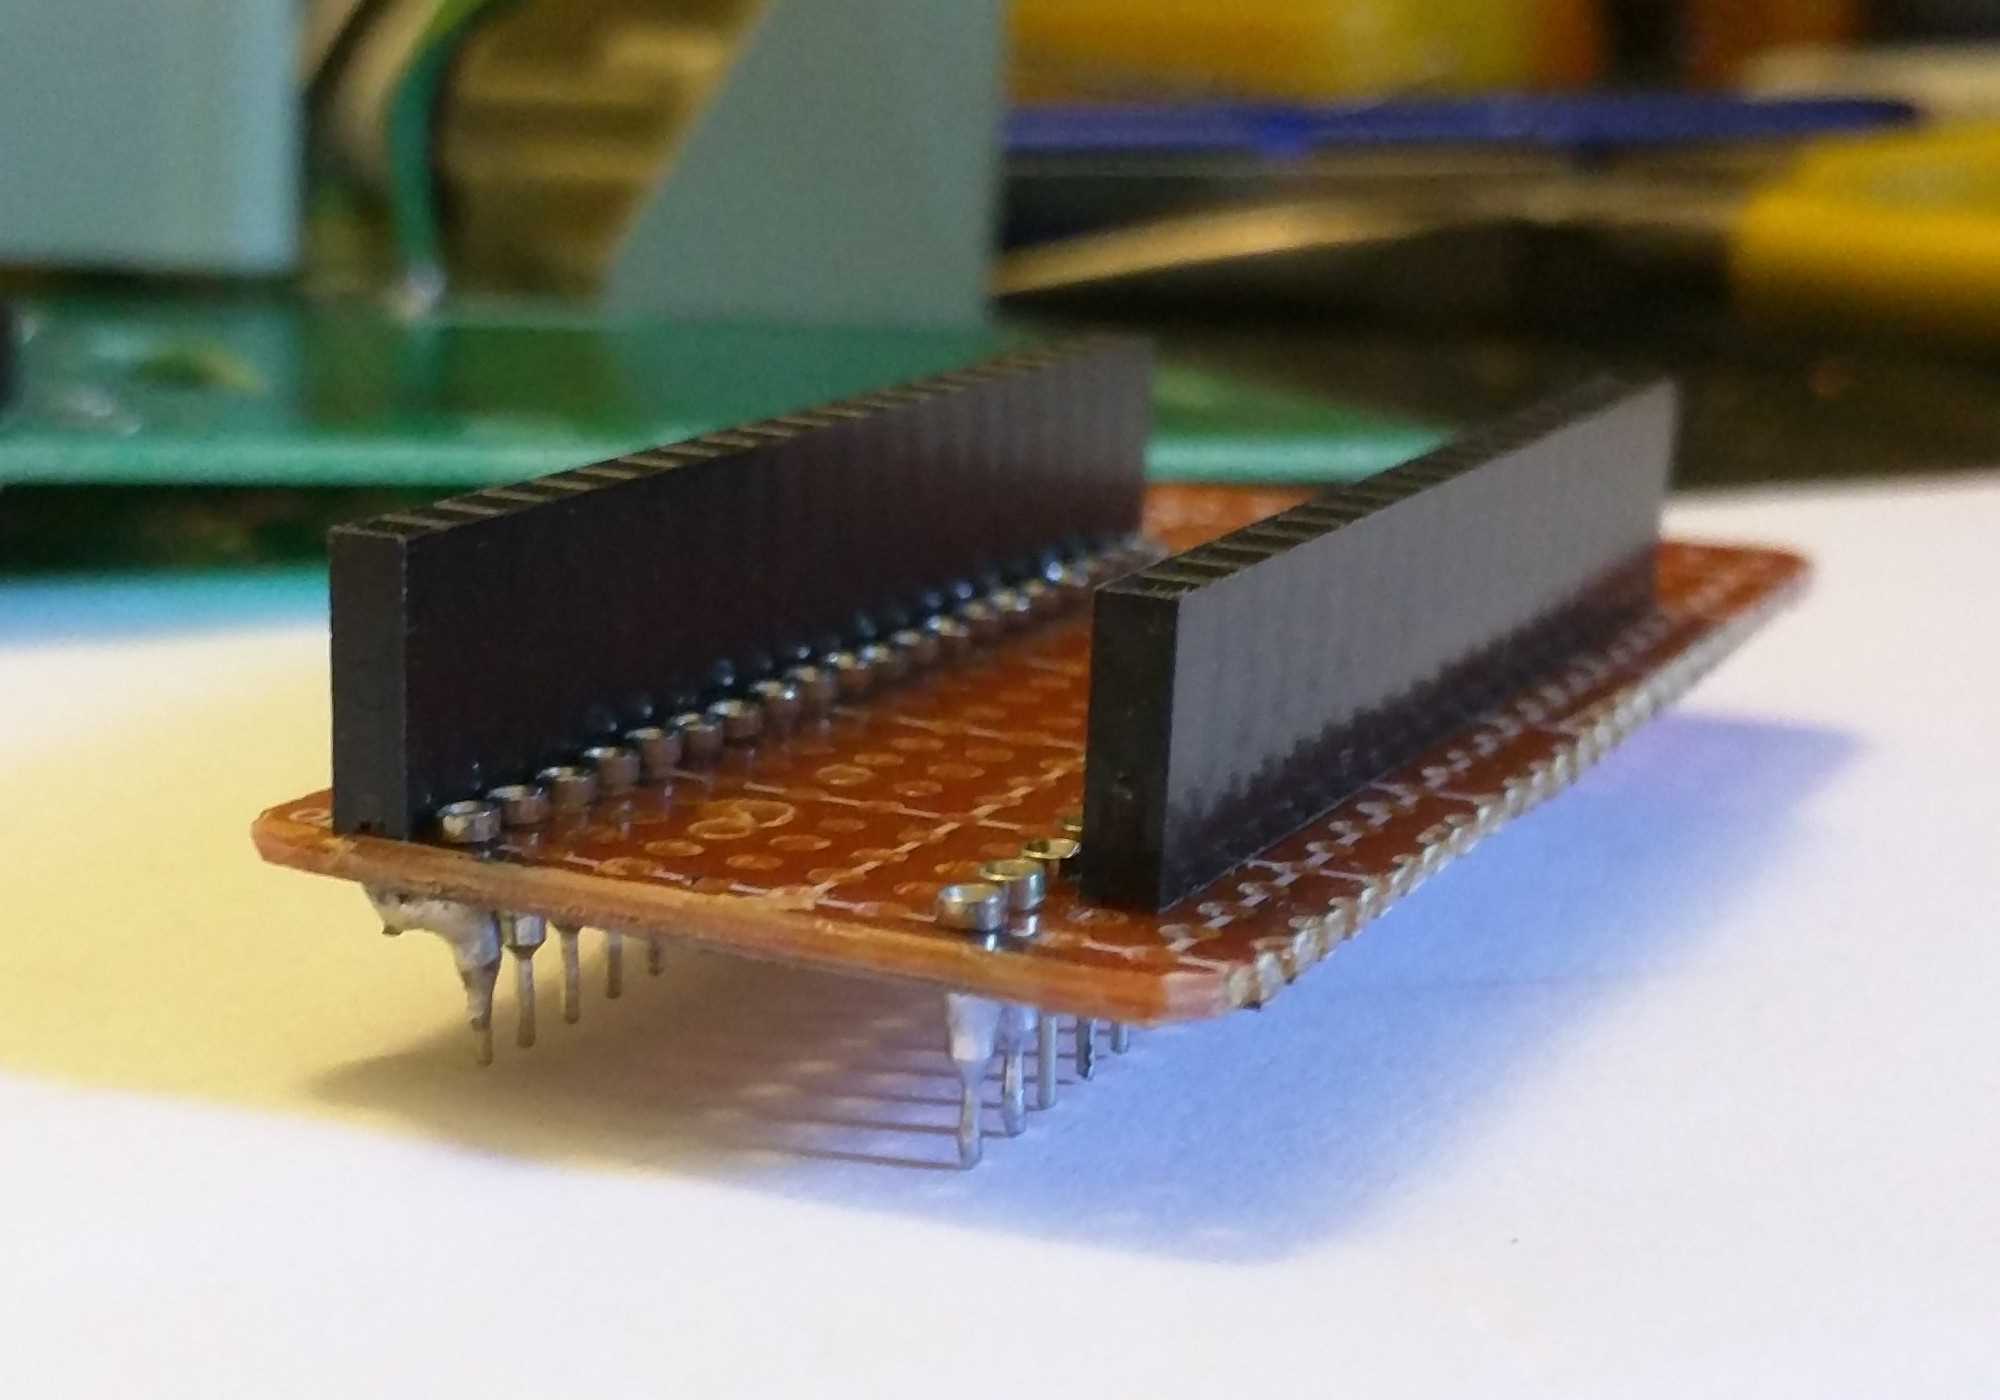
\includegraphics[width=0.60\linewidth]{figures/pic-u17-piggybacked-side.jpg}
    \caption{The Fluke8050a U17 piggybacked board.} \label{fig:picf8050apiggybrd}
\end{figure}




\begin{figure}[h!t] \centering
    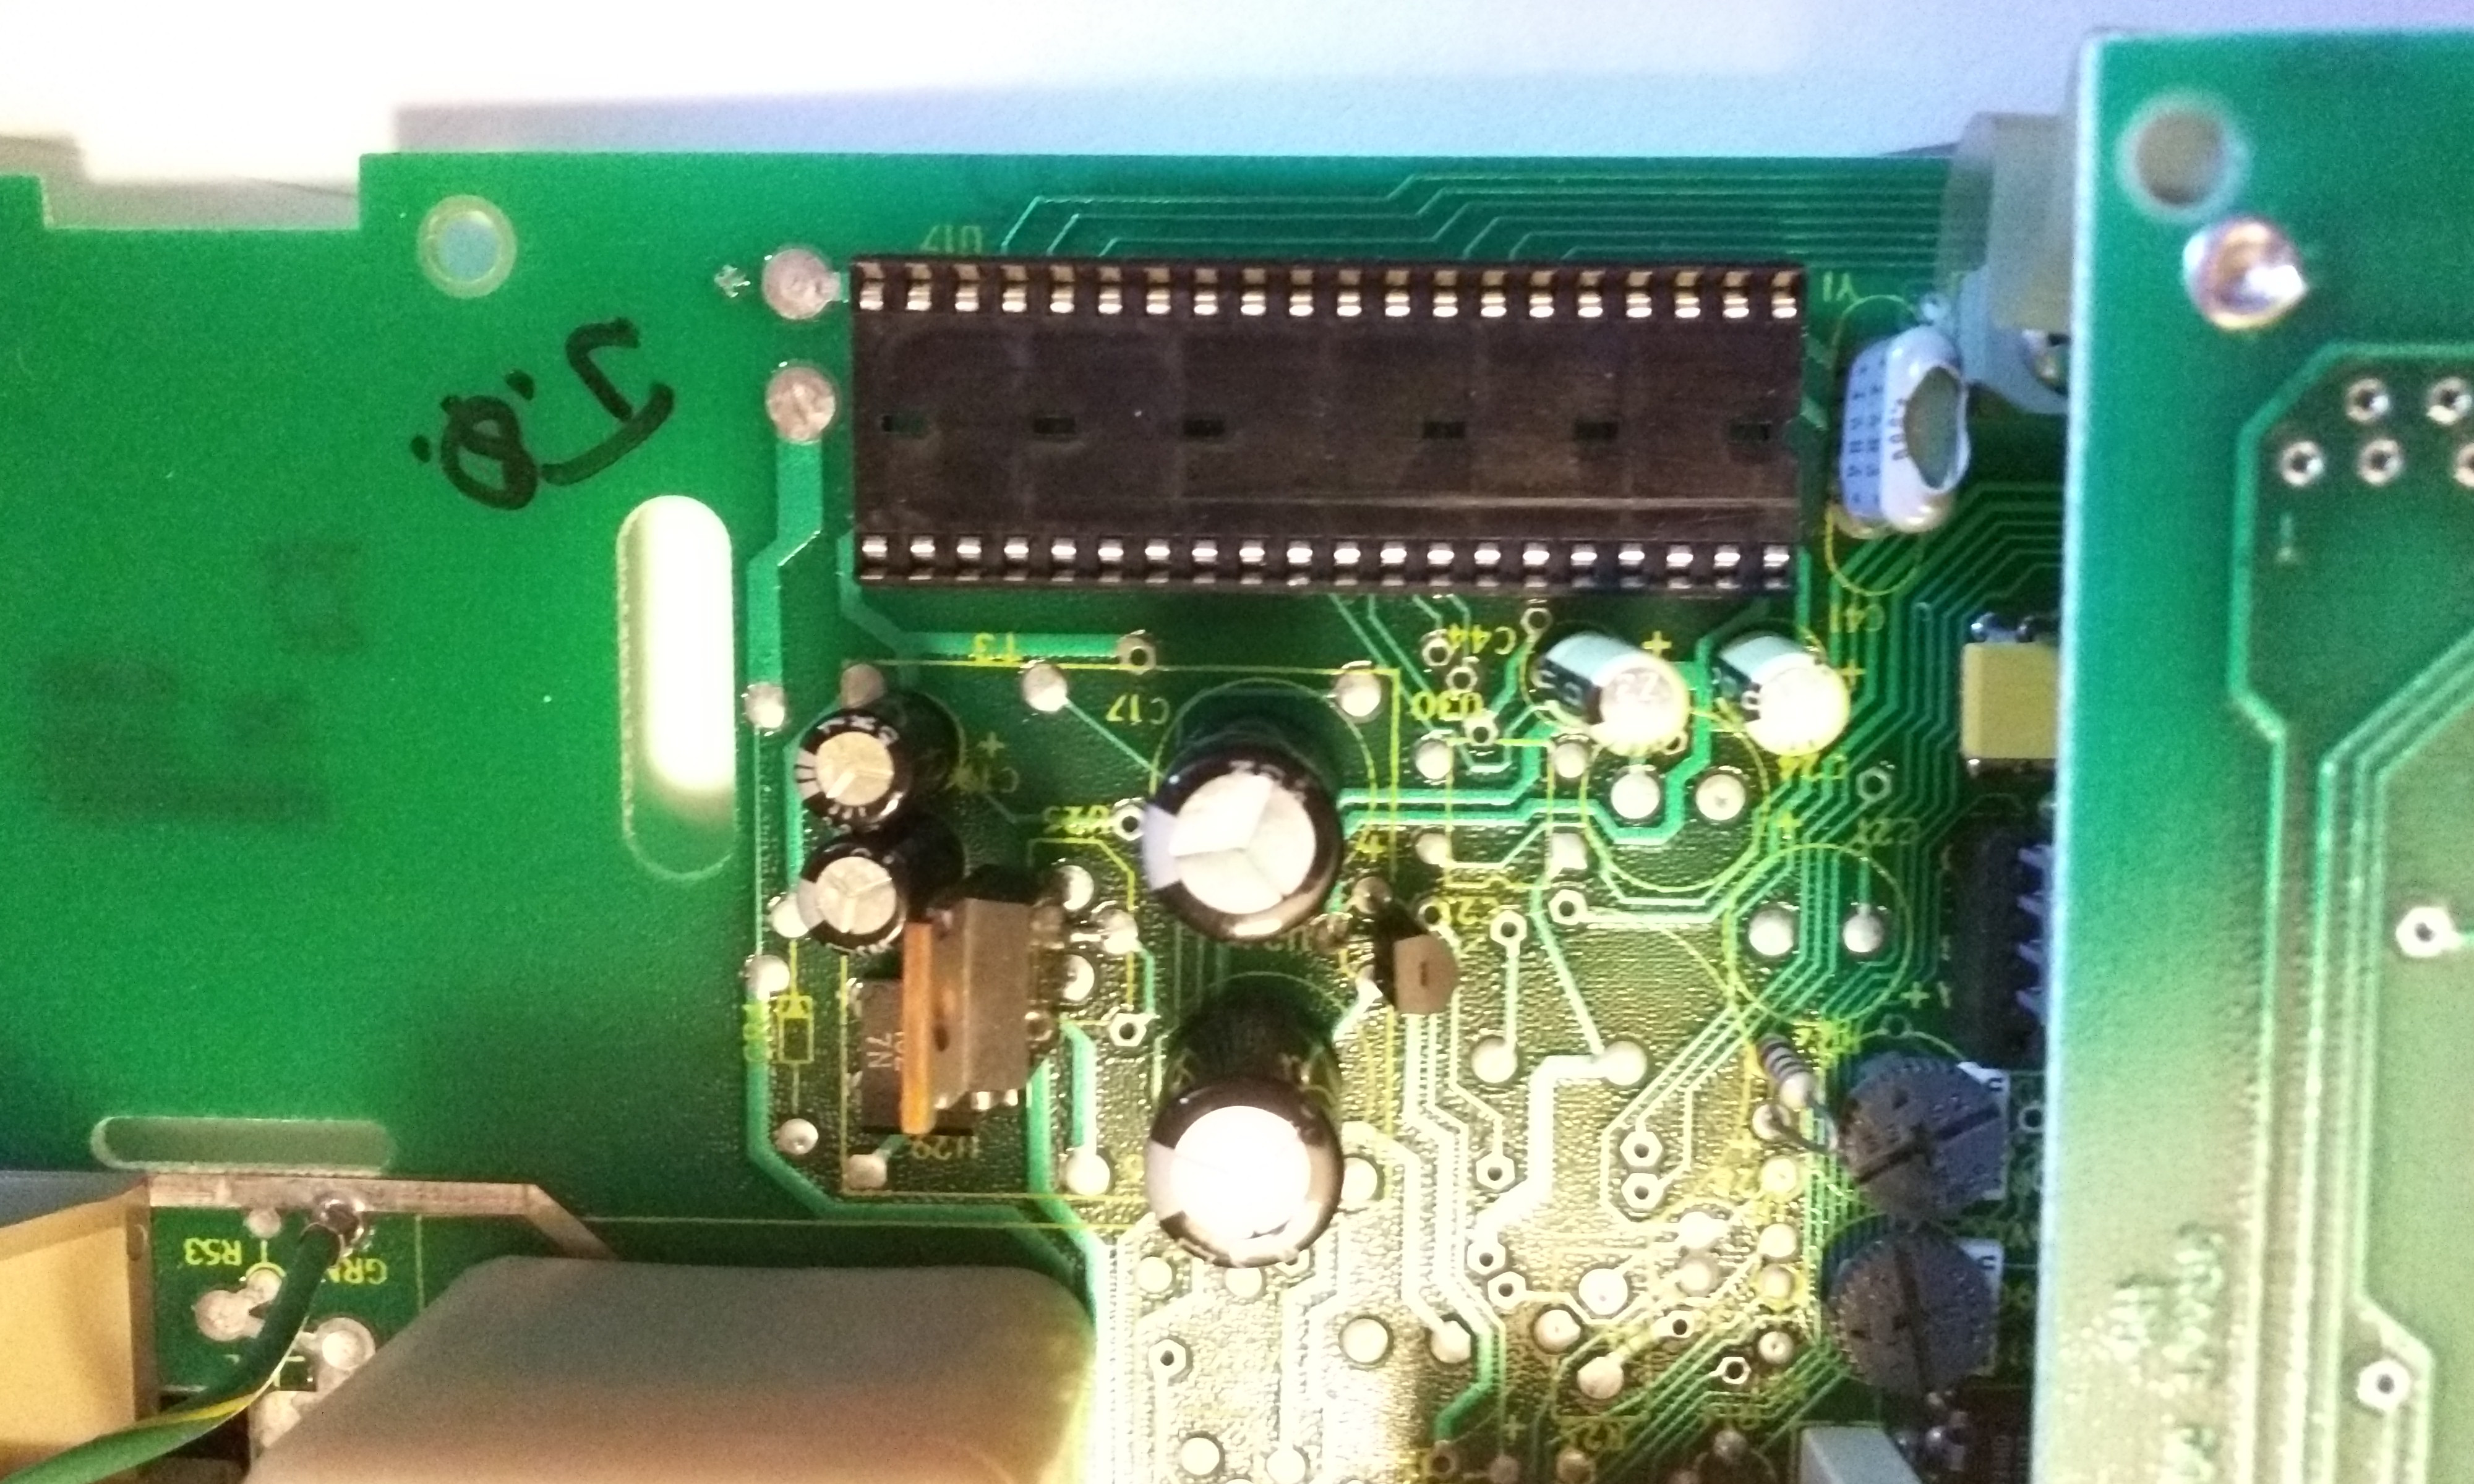
\includegraphics[width=0.45\linewidth]{figures/pic-u17-origin.jpg}
    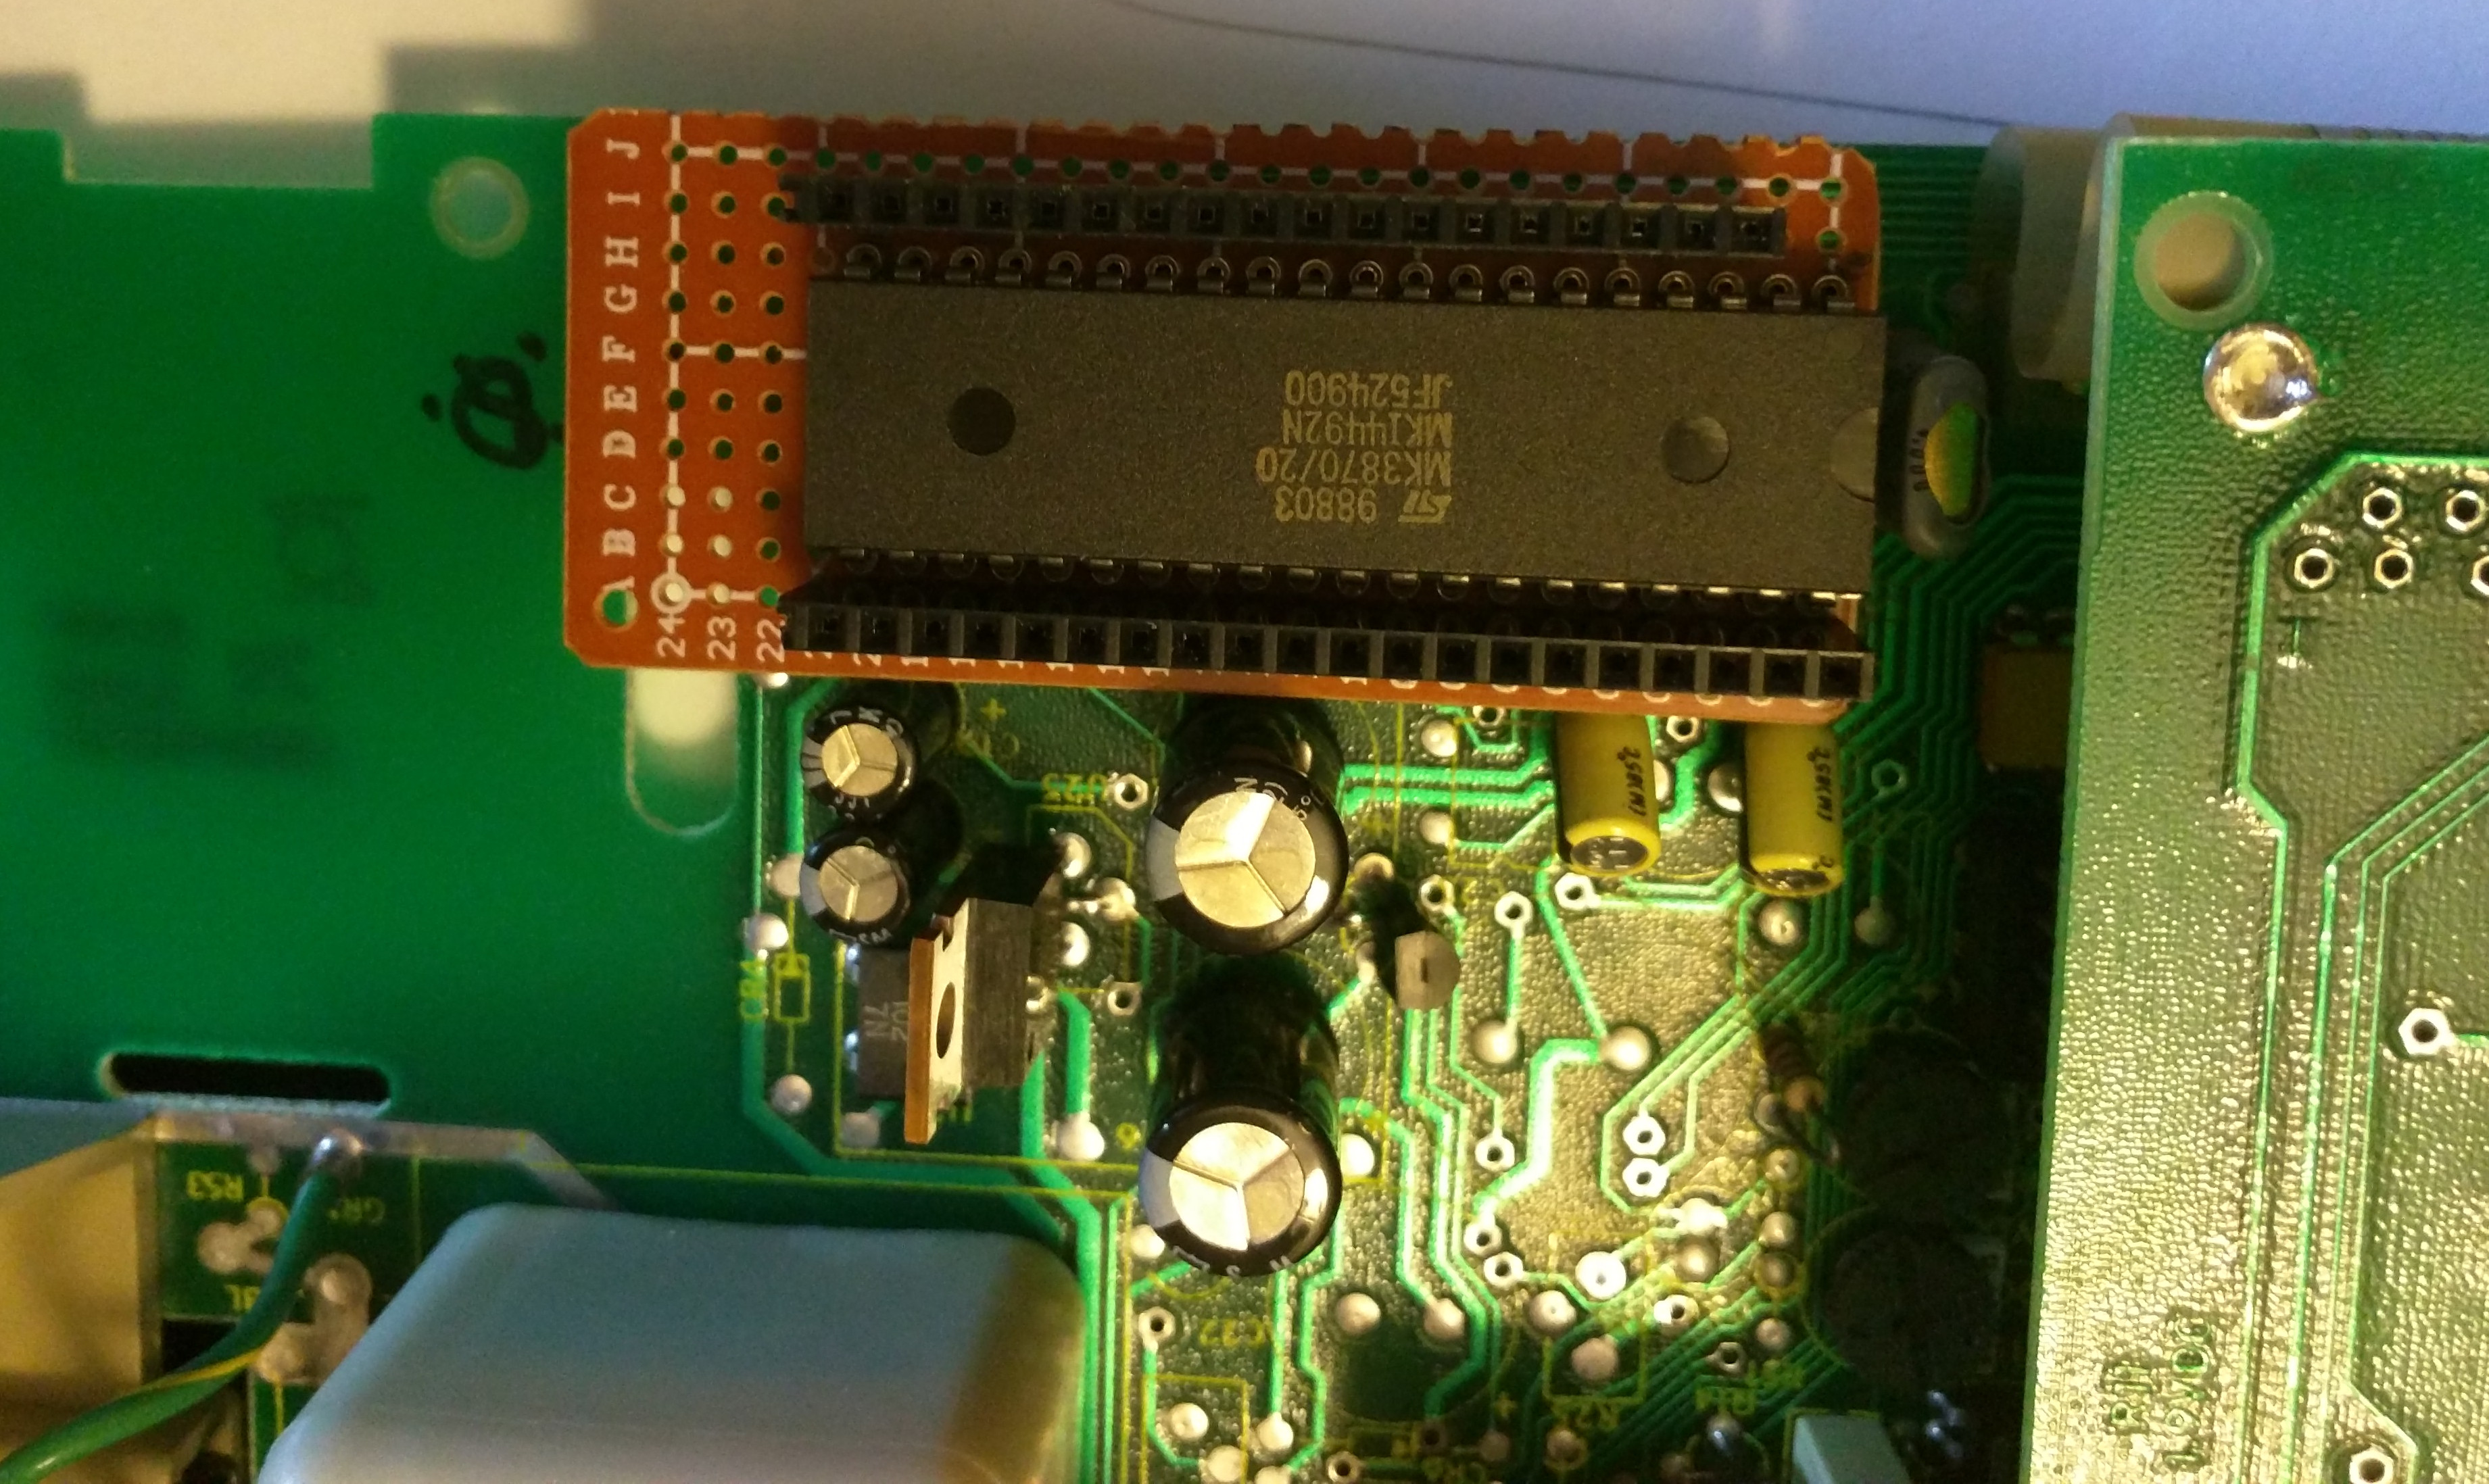
\includegraphics[width=0.45\linewidth]{figures/pic-u17-piggybacked-1.jpg}
    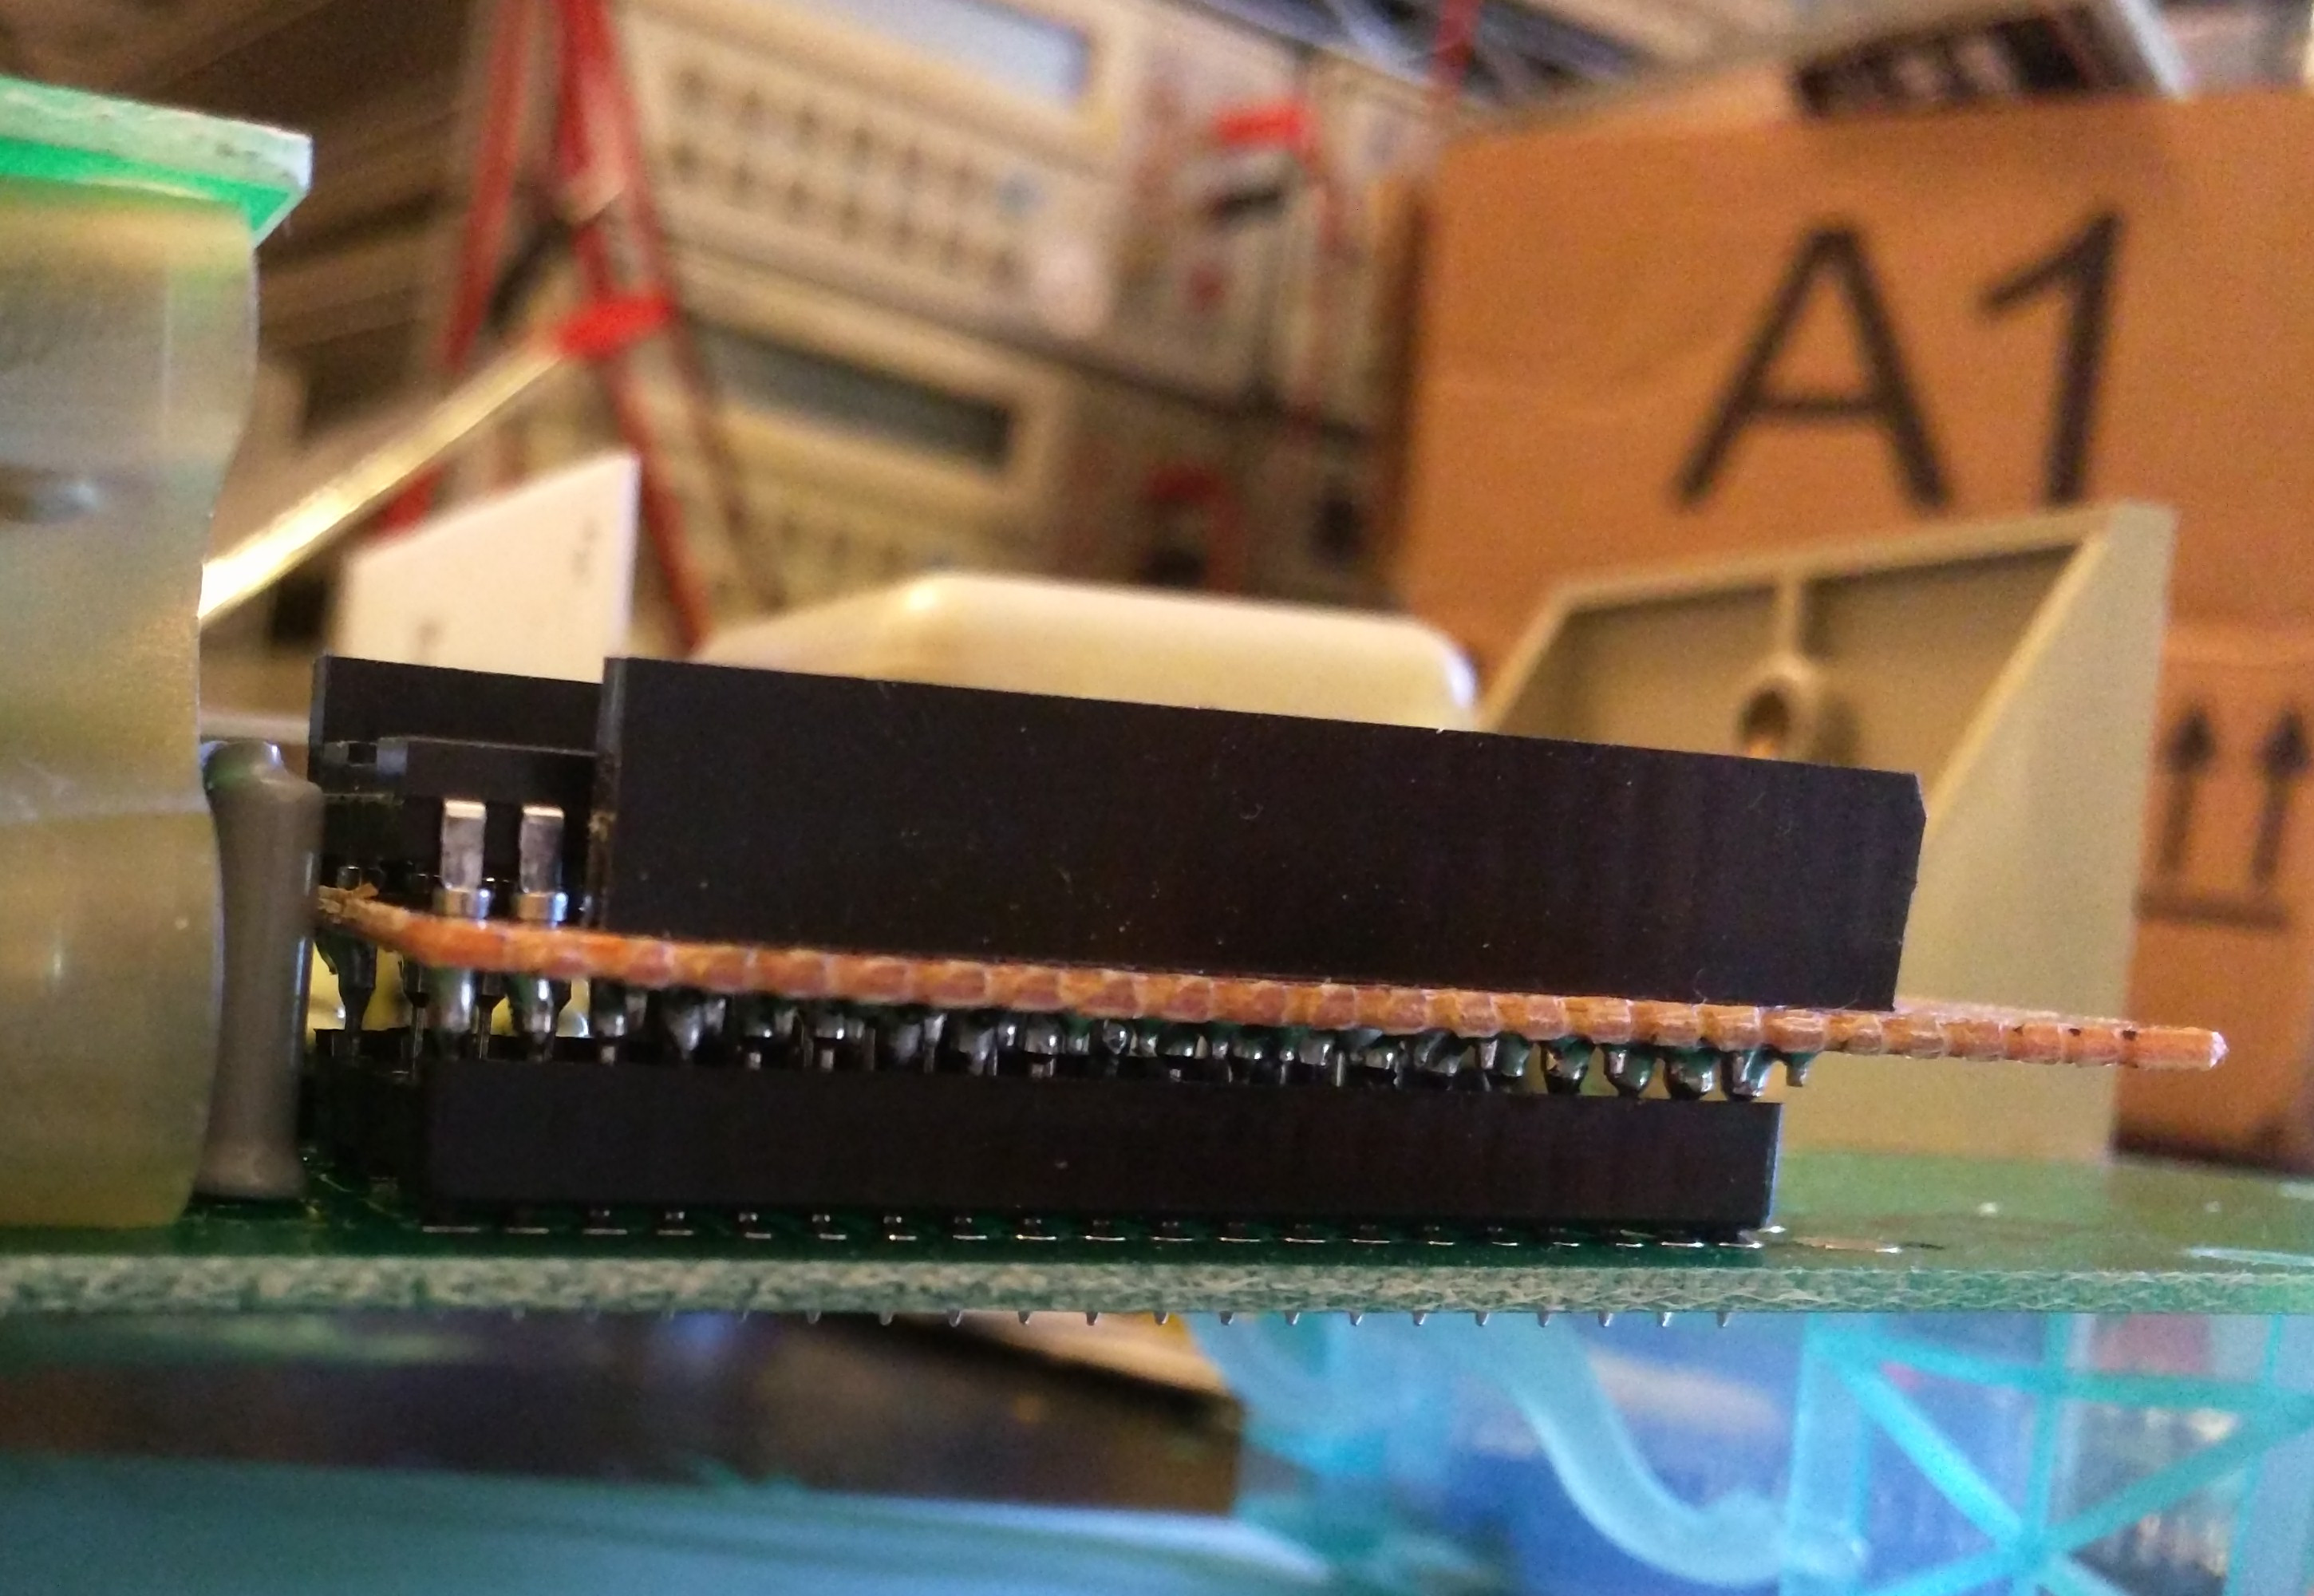
\includegraphics[width=0.45\linewidth]{figures/pic-u17-piggybacked-2.jpg}
    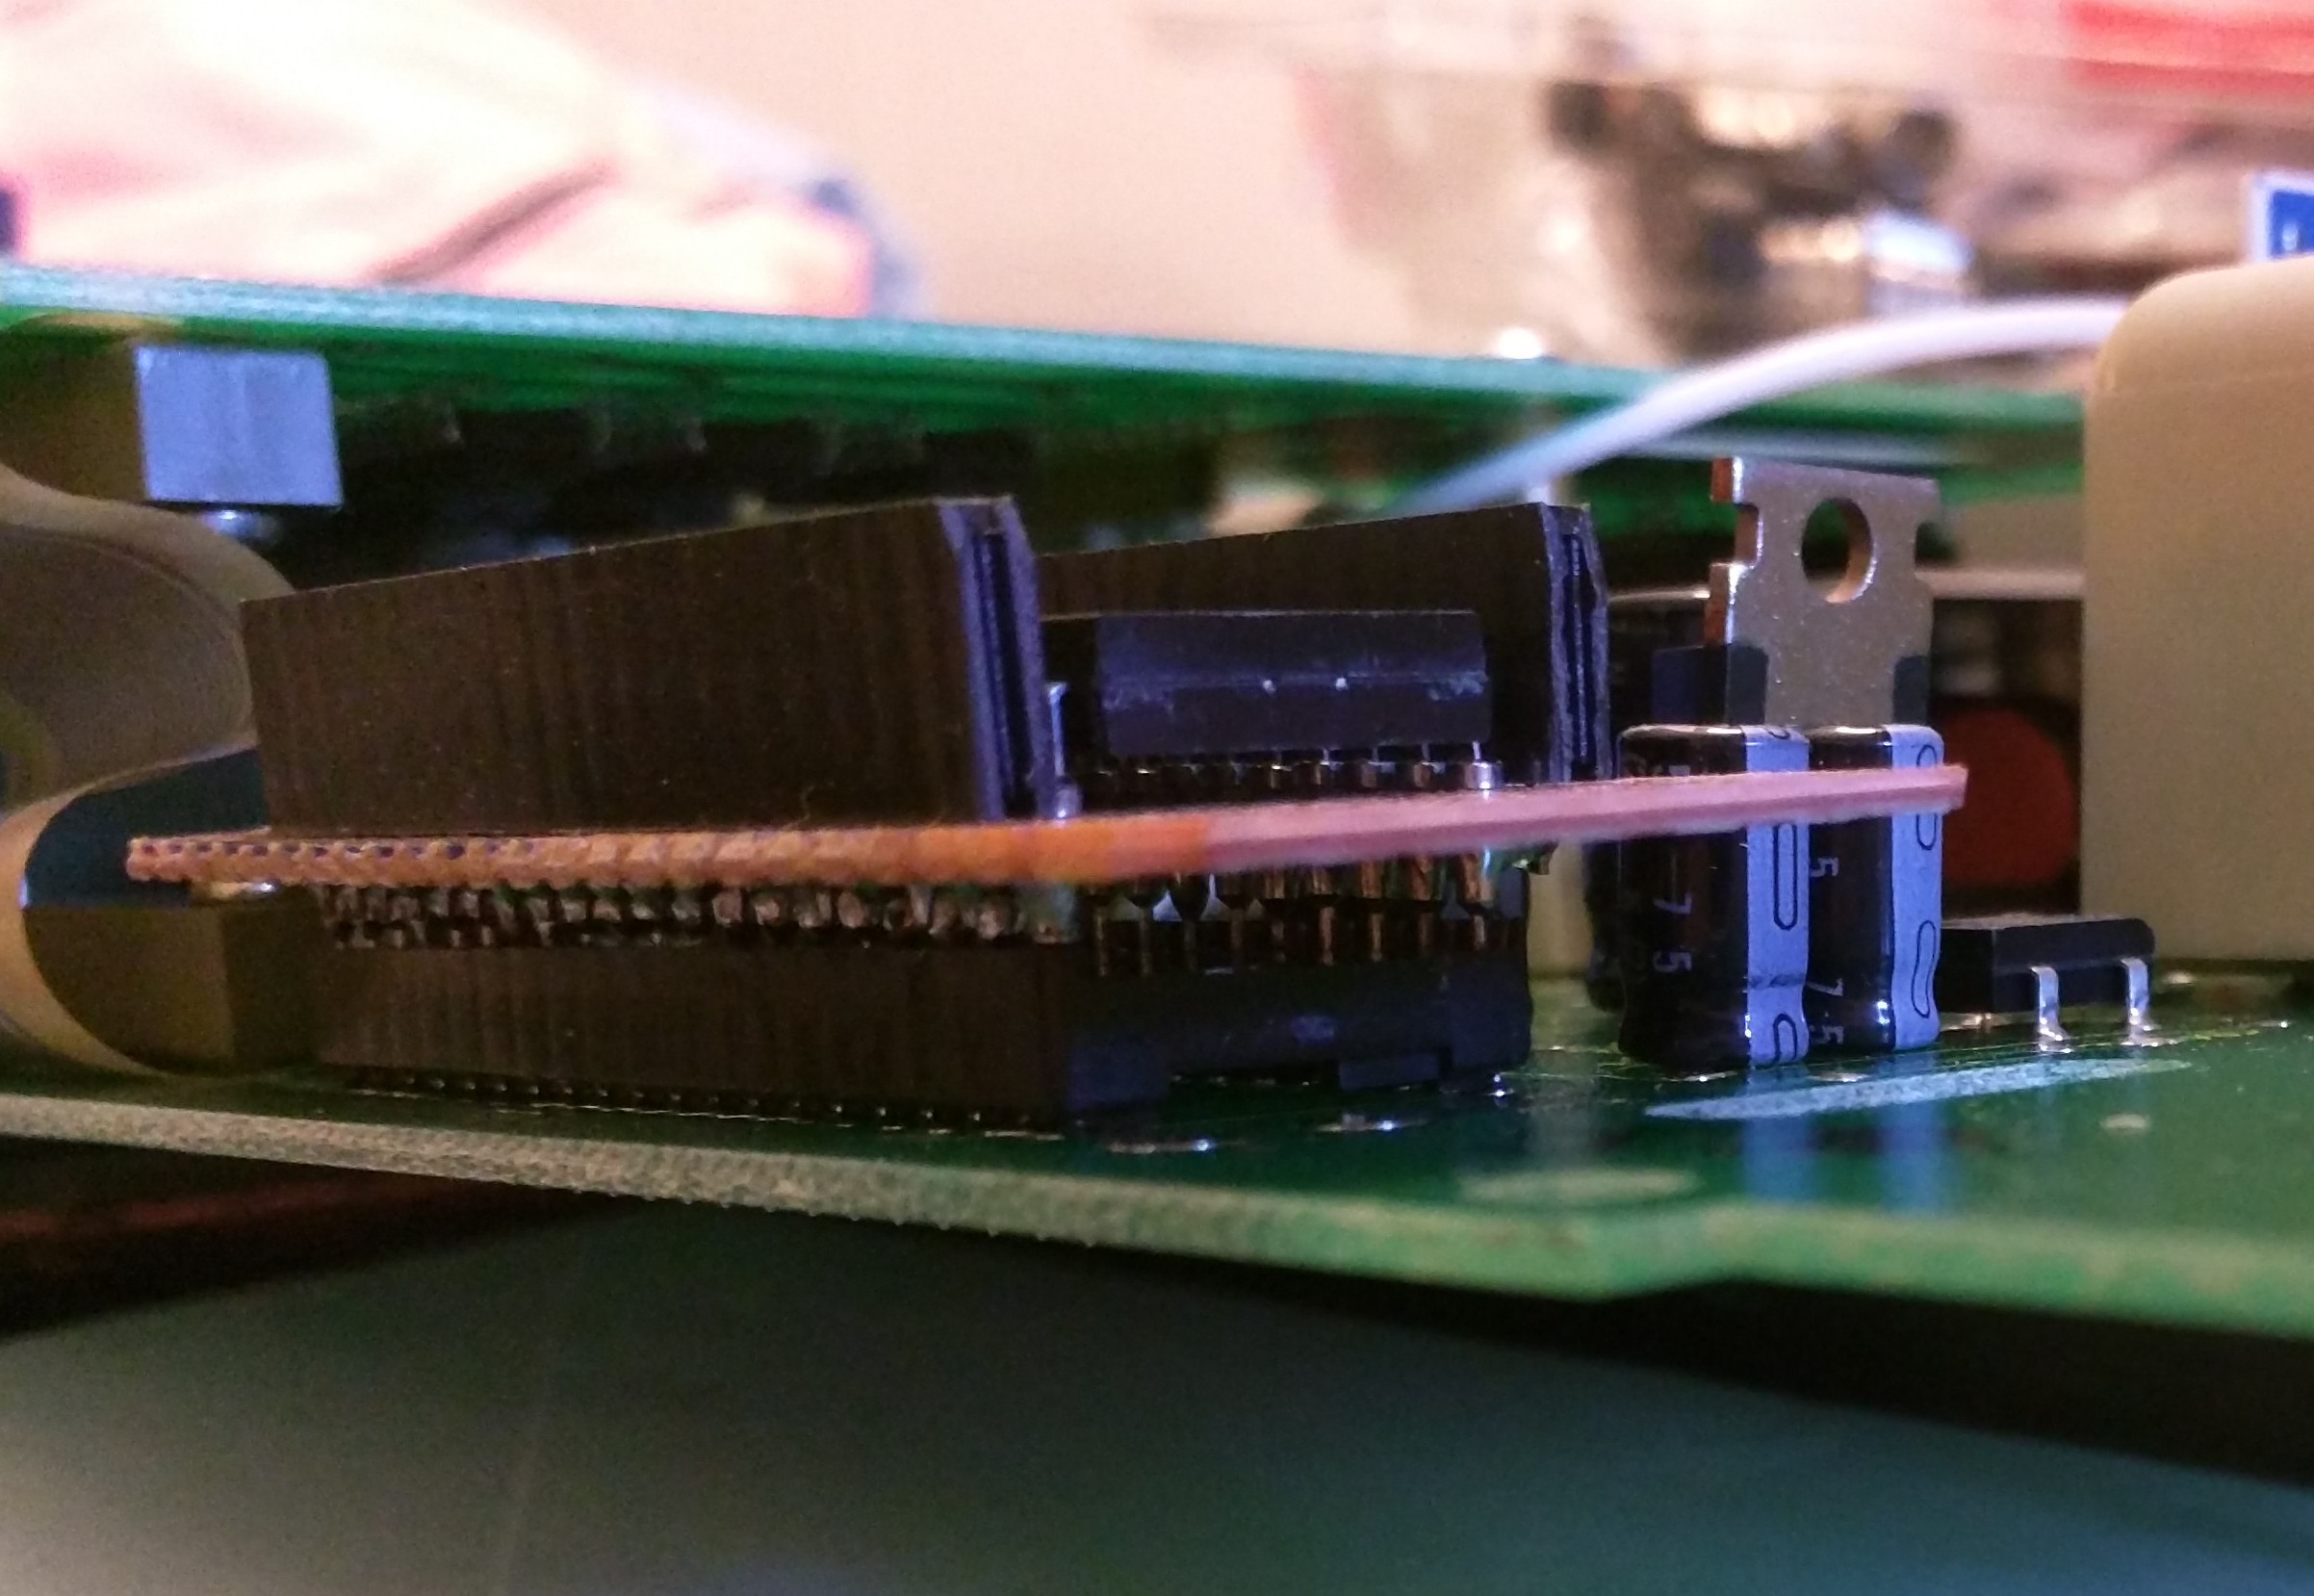
\includegraphics[width=0.45\linewidth]{figures/pic-u17-piggybacked-3.jpg}
    \caption{The Fluke8050a U17 piggybacked board installed.} \label{fig:picf8050apiggy}
\end{figure}






\begin{figure}[h!t] \centering
    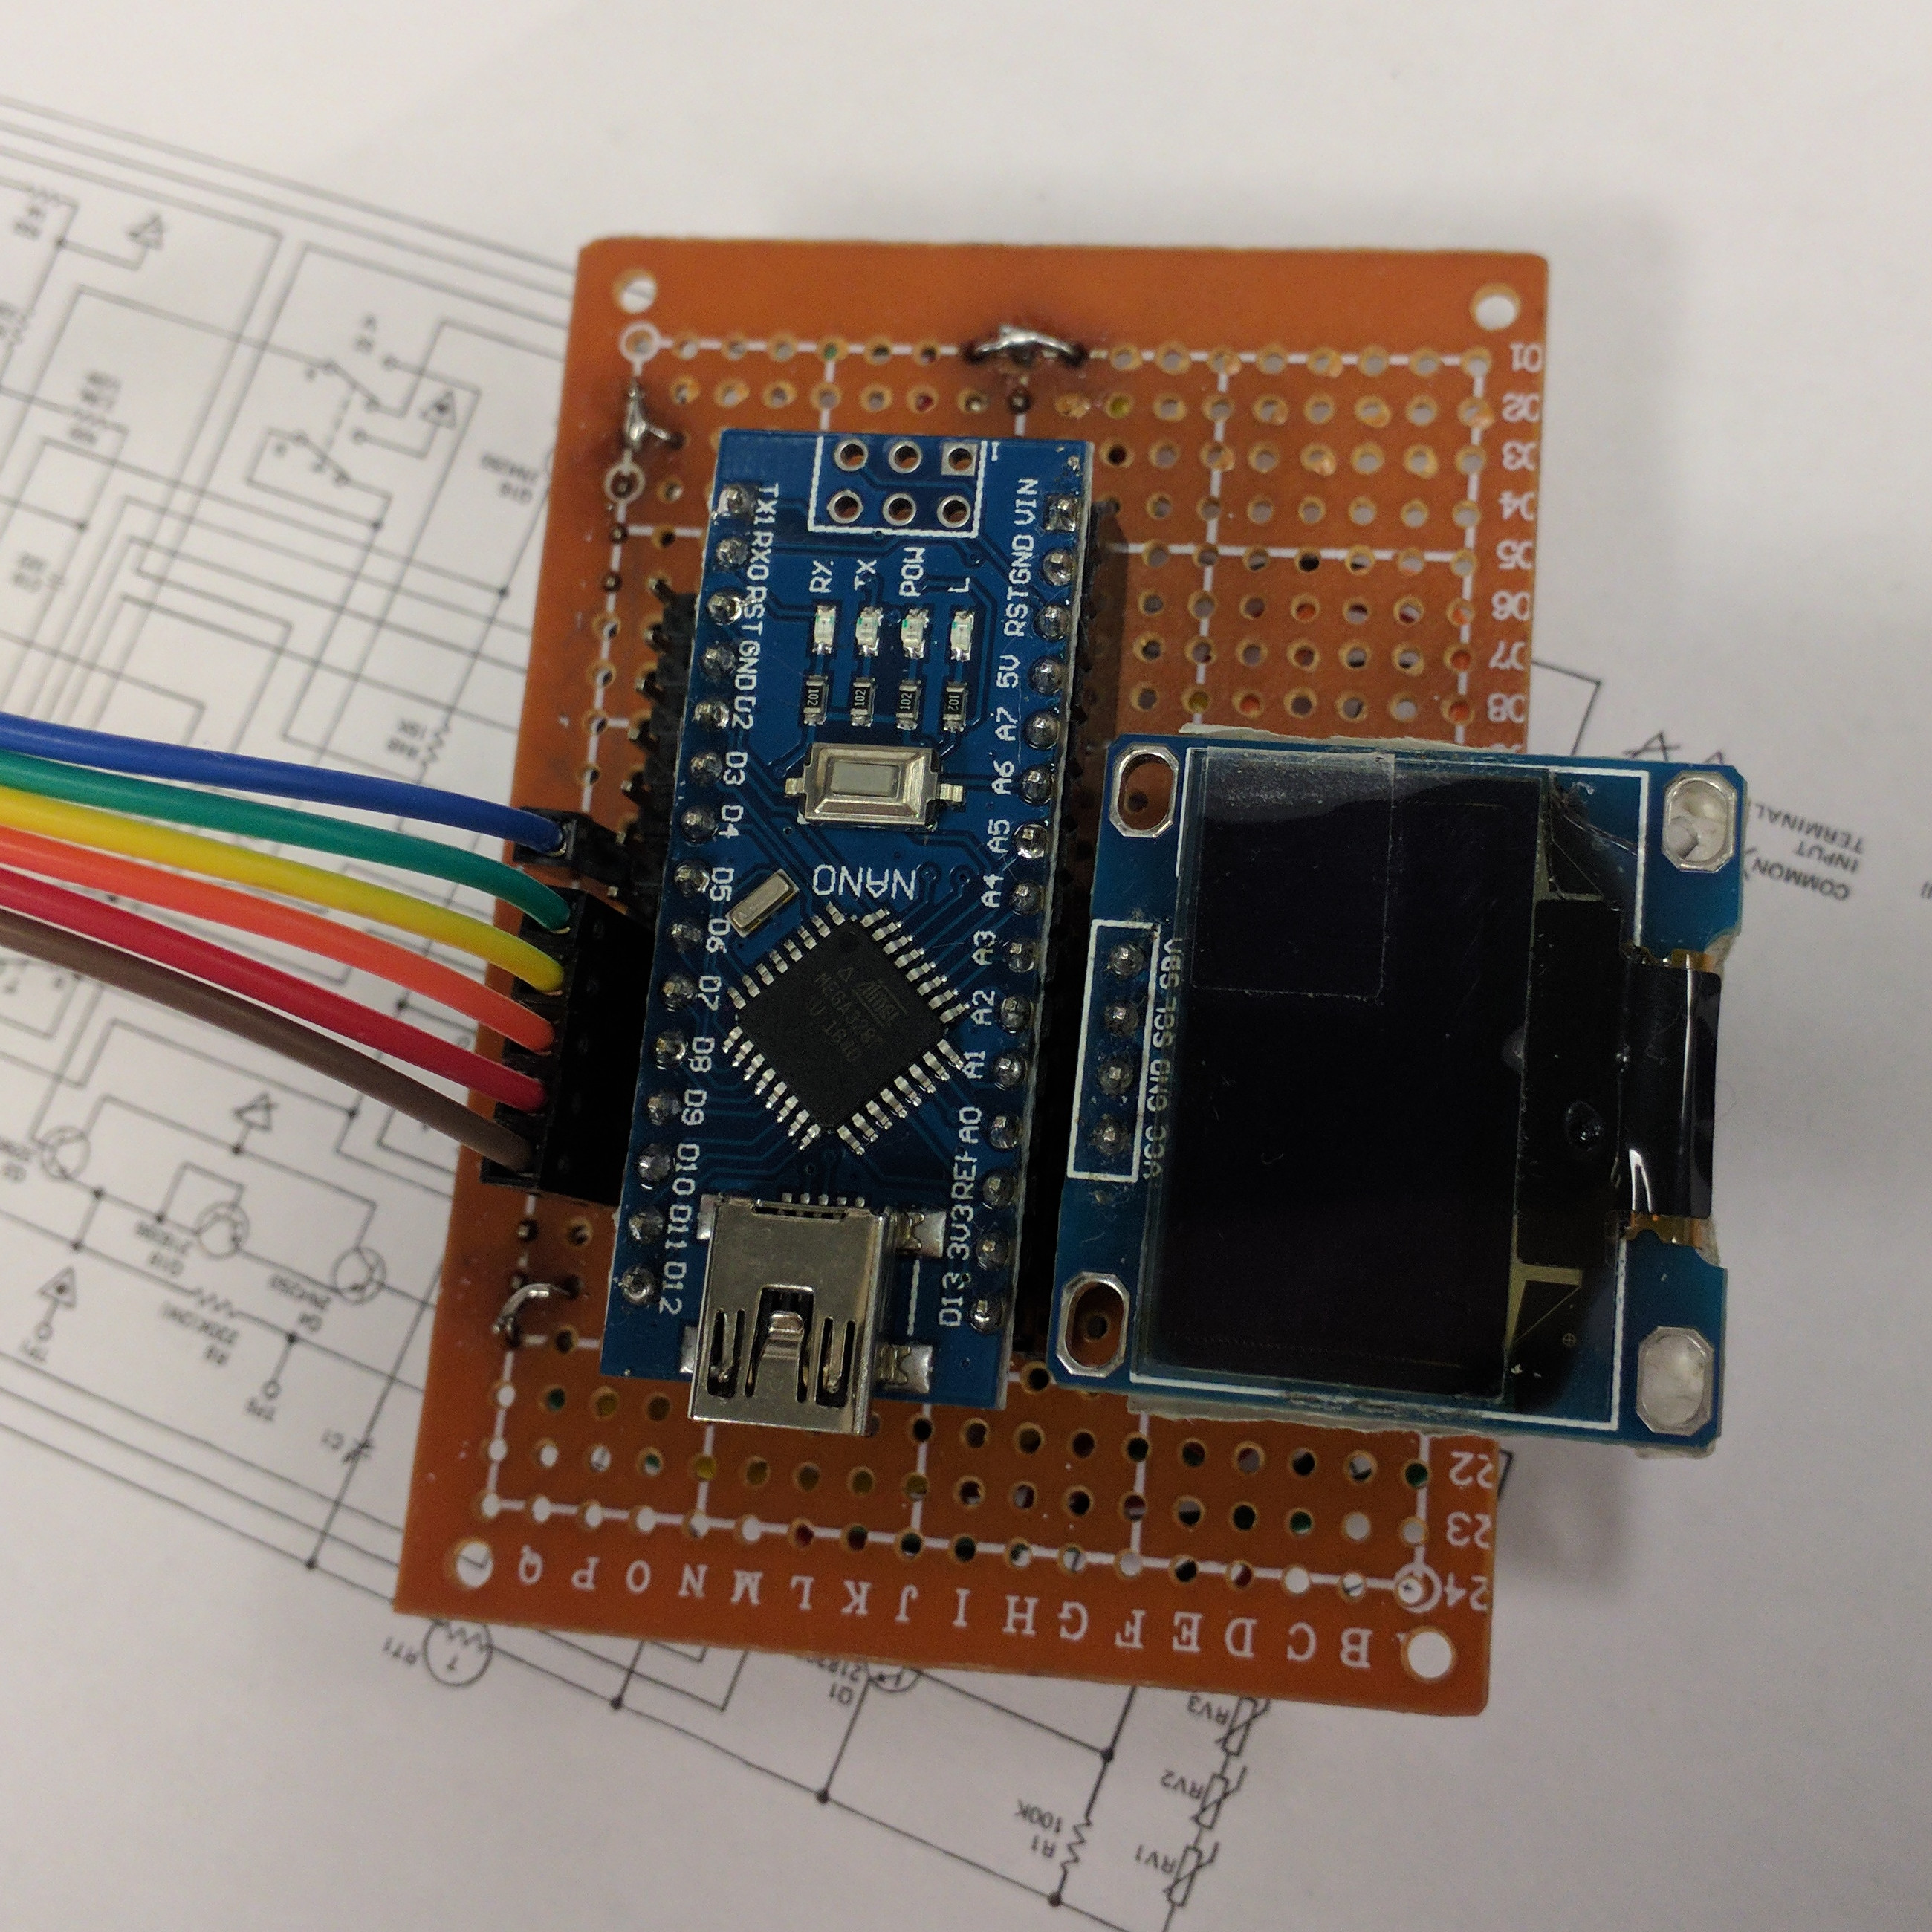
\includegraphics[width=0.45\linewidth]{figures/pic-smartshow-closer-main.jpg}
    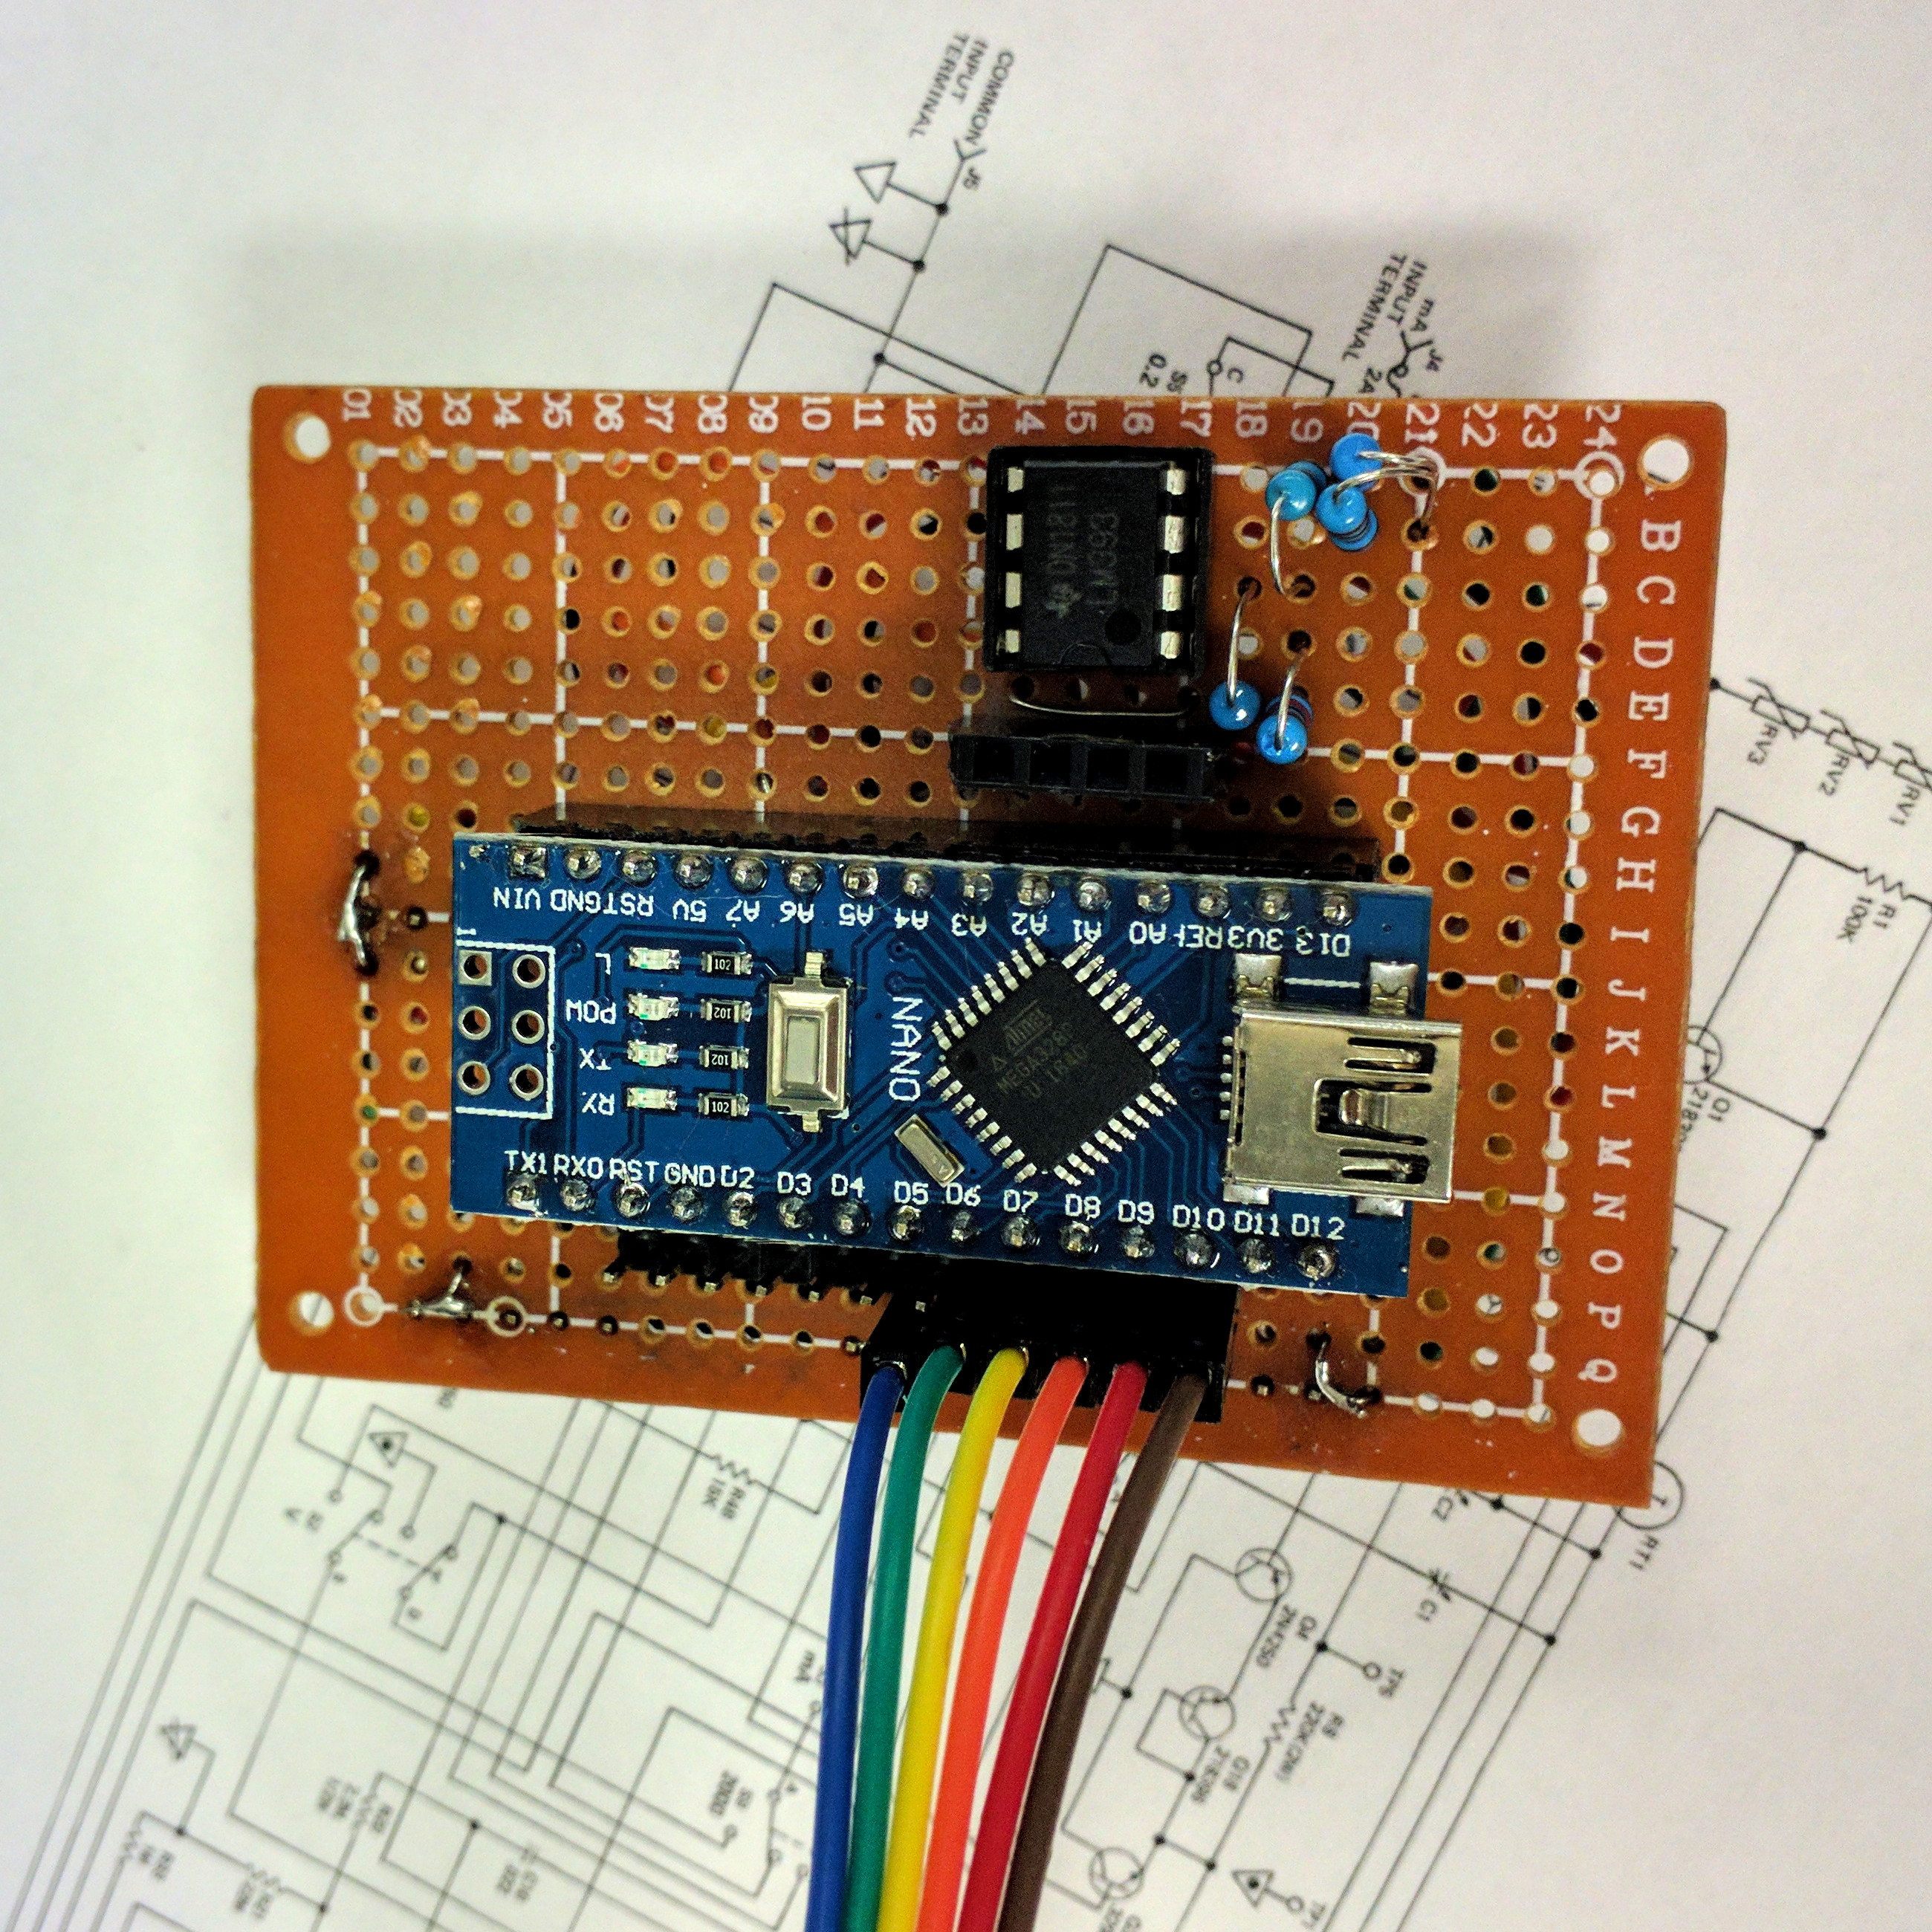
\includegraphics[width=0.45\linewidth]{figures/pic-smartshow-closer-main-nooled.jpg}
    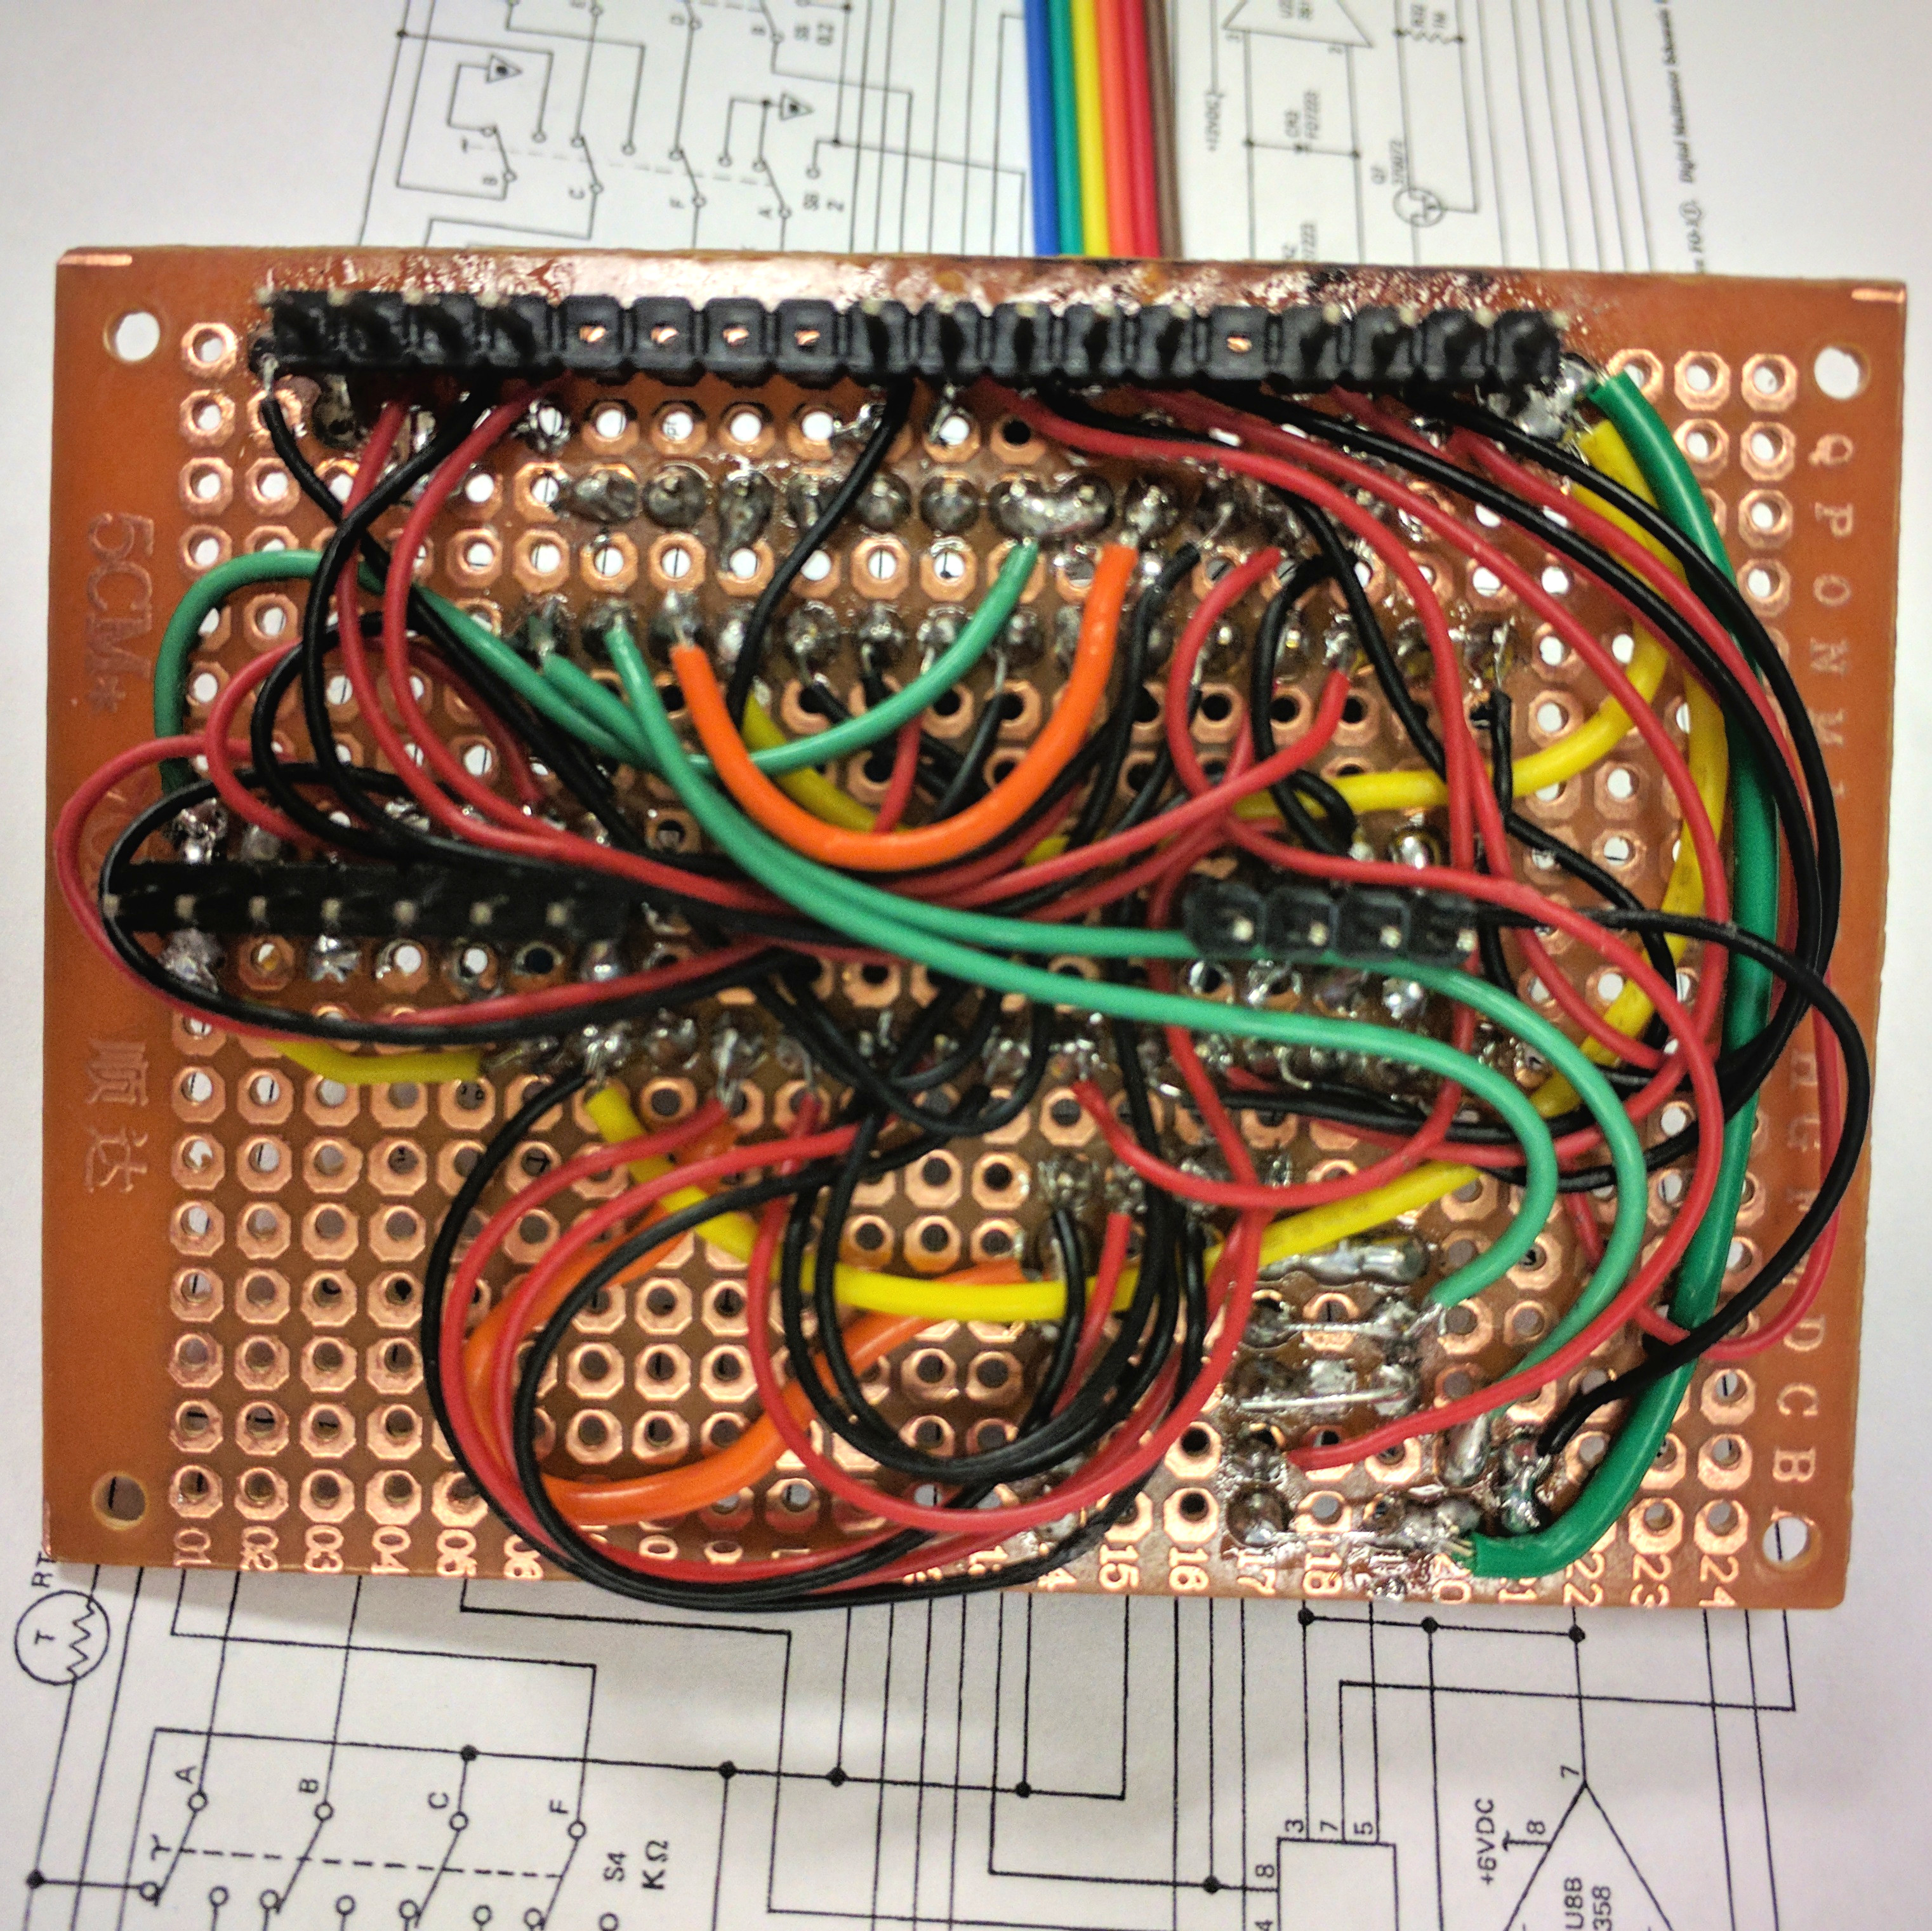
\includegraphics[width=0.45\linewidth]{figures/pic-smartshow-closer-main-back.jpg}
    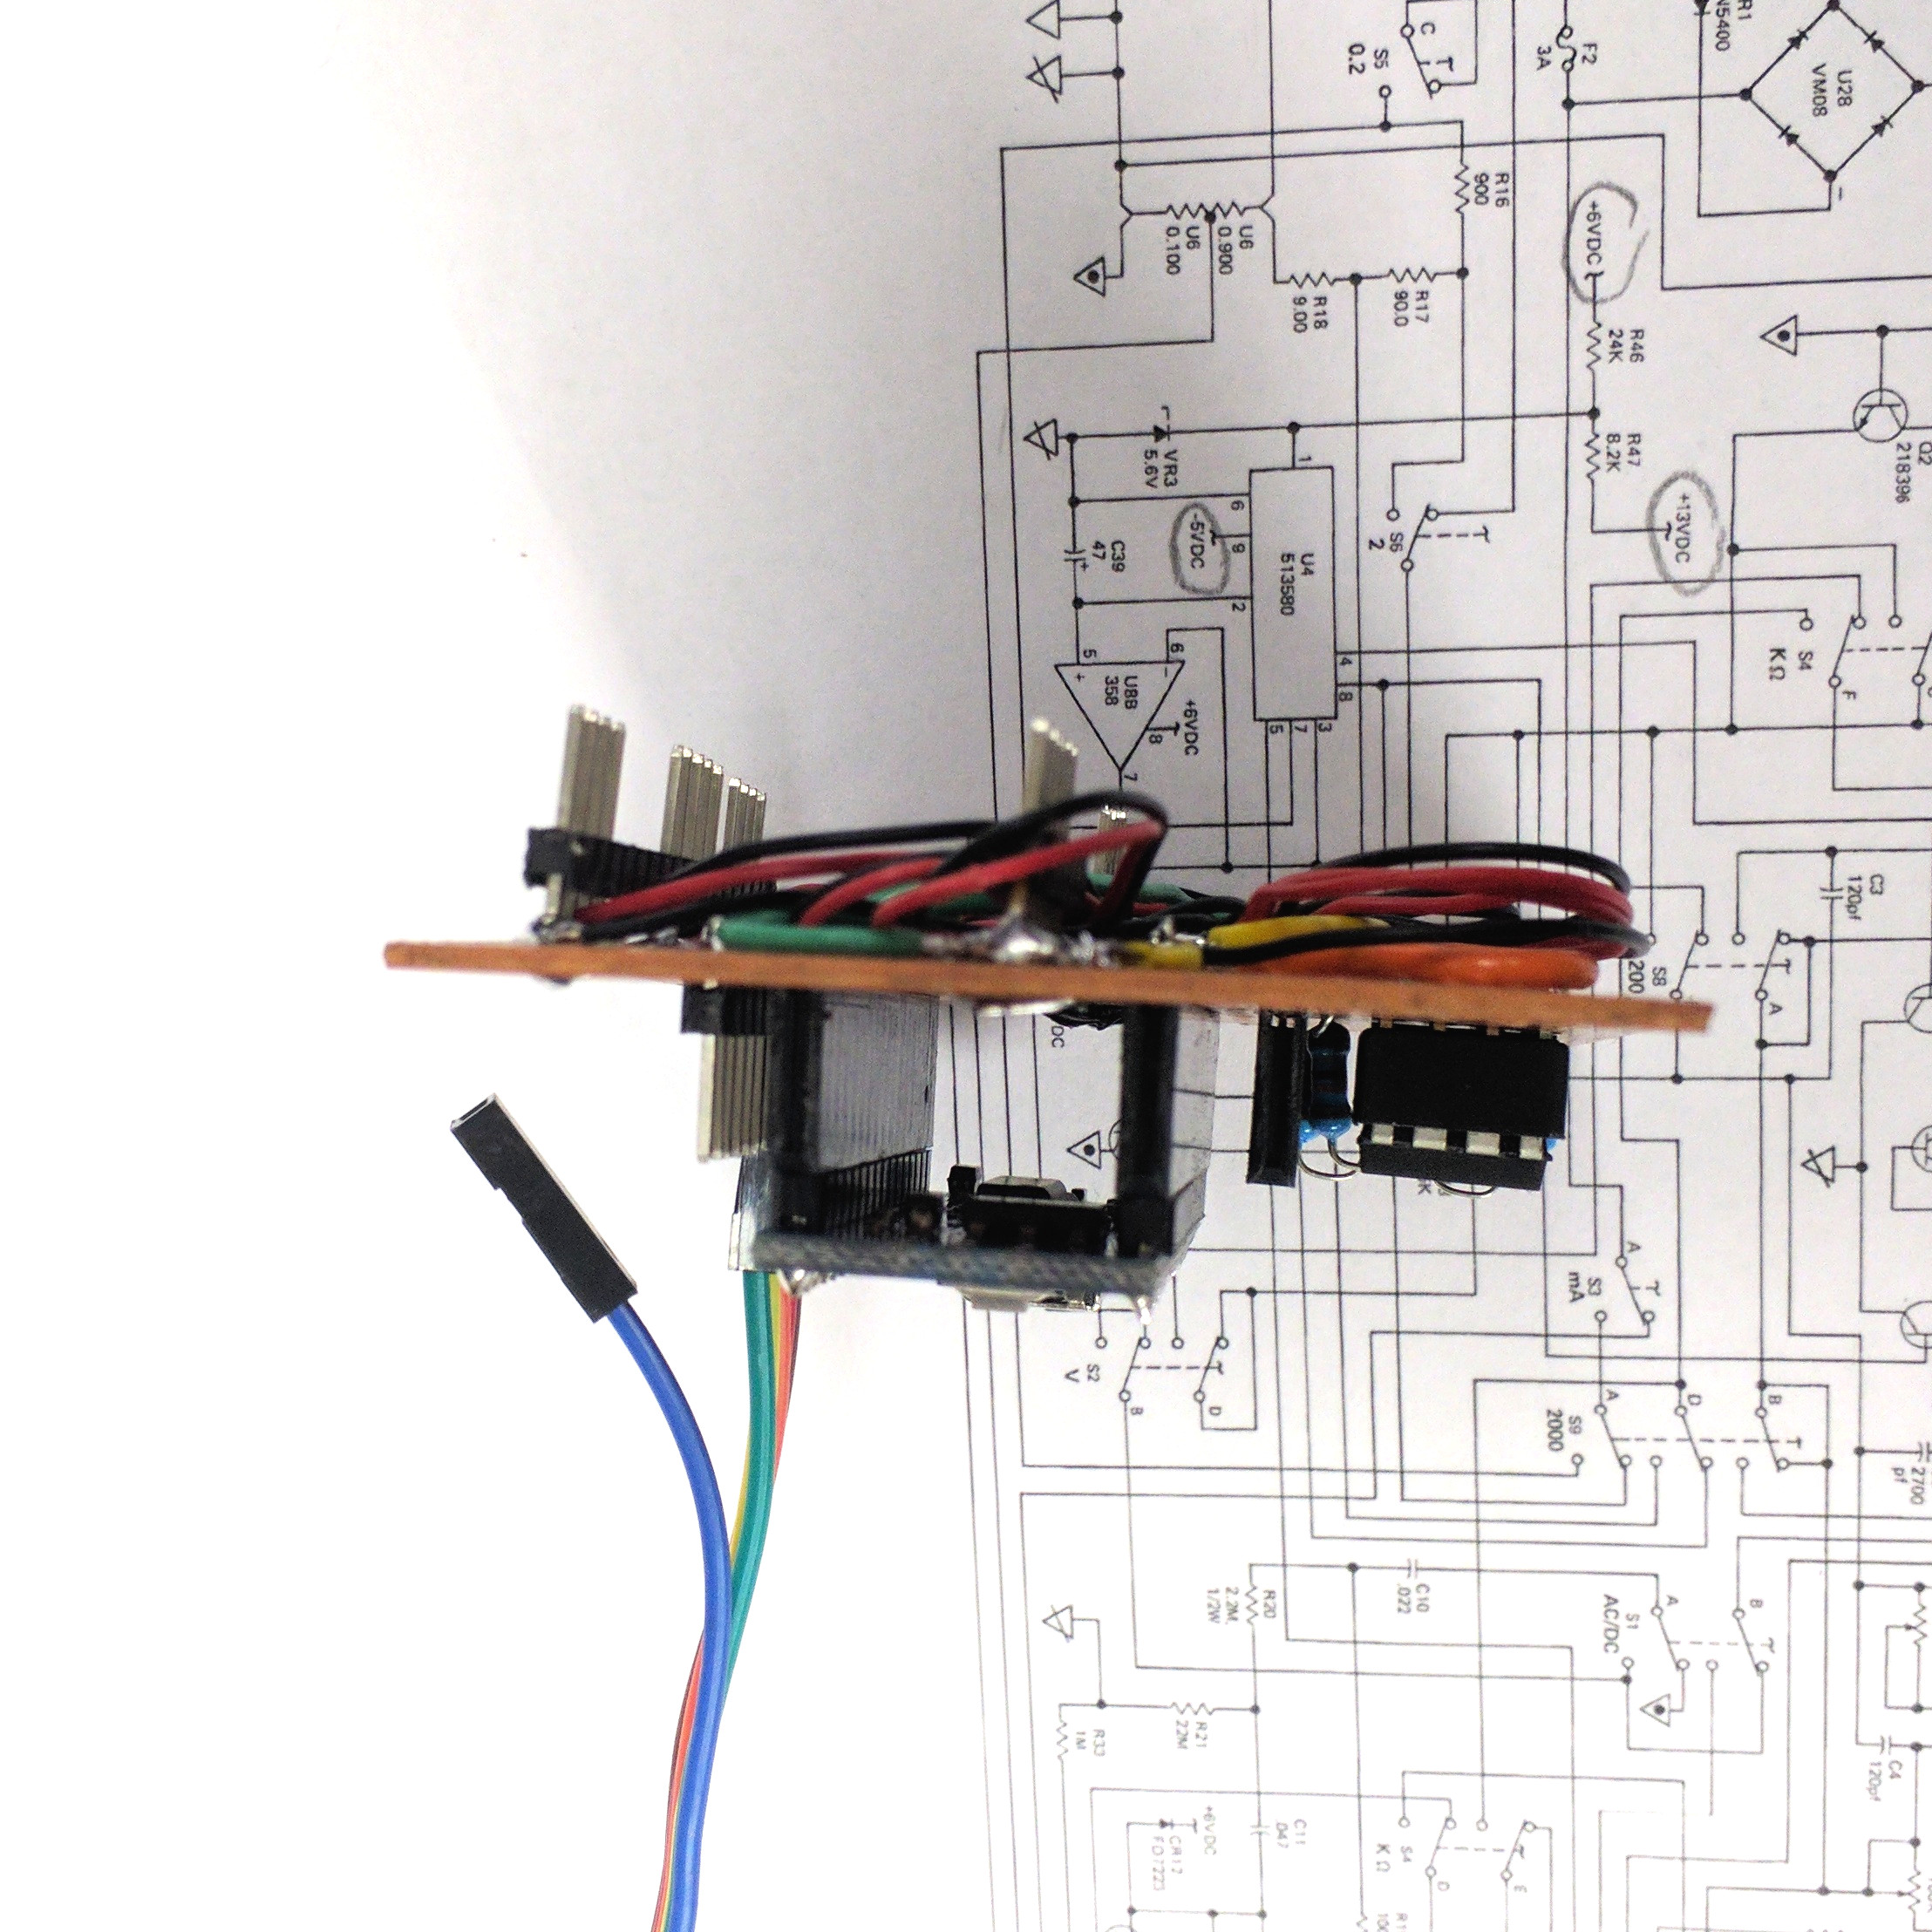
\includegraphics[width=0.45\linewidth]{figures/pic-smartshow-closer-main-side.jpg}
    \caption{The SmartShow main board.} \label{fig:picsmmain}
\end{figure}


\begin{figure}[h!t] \centering
    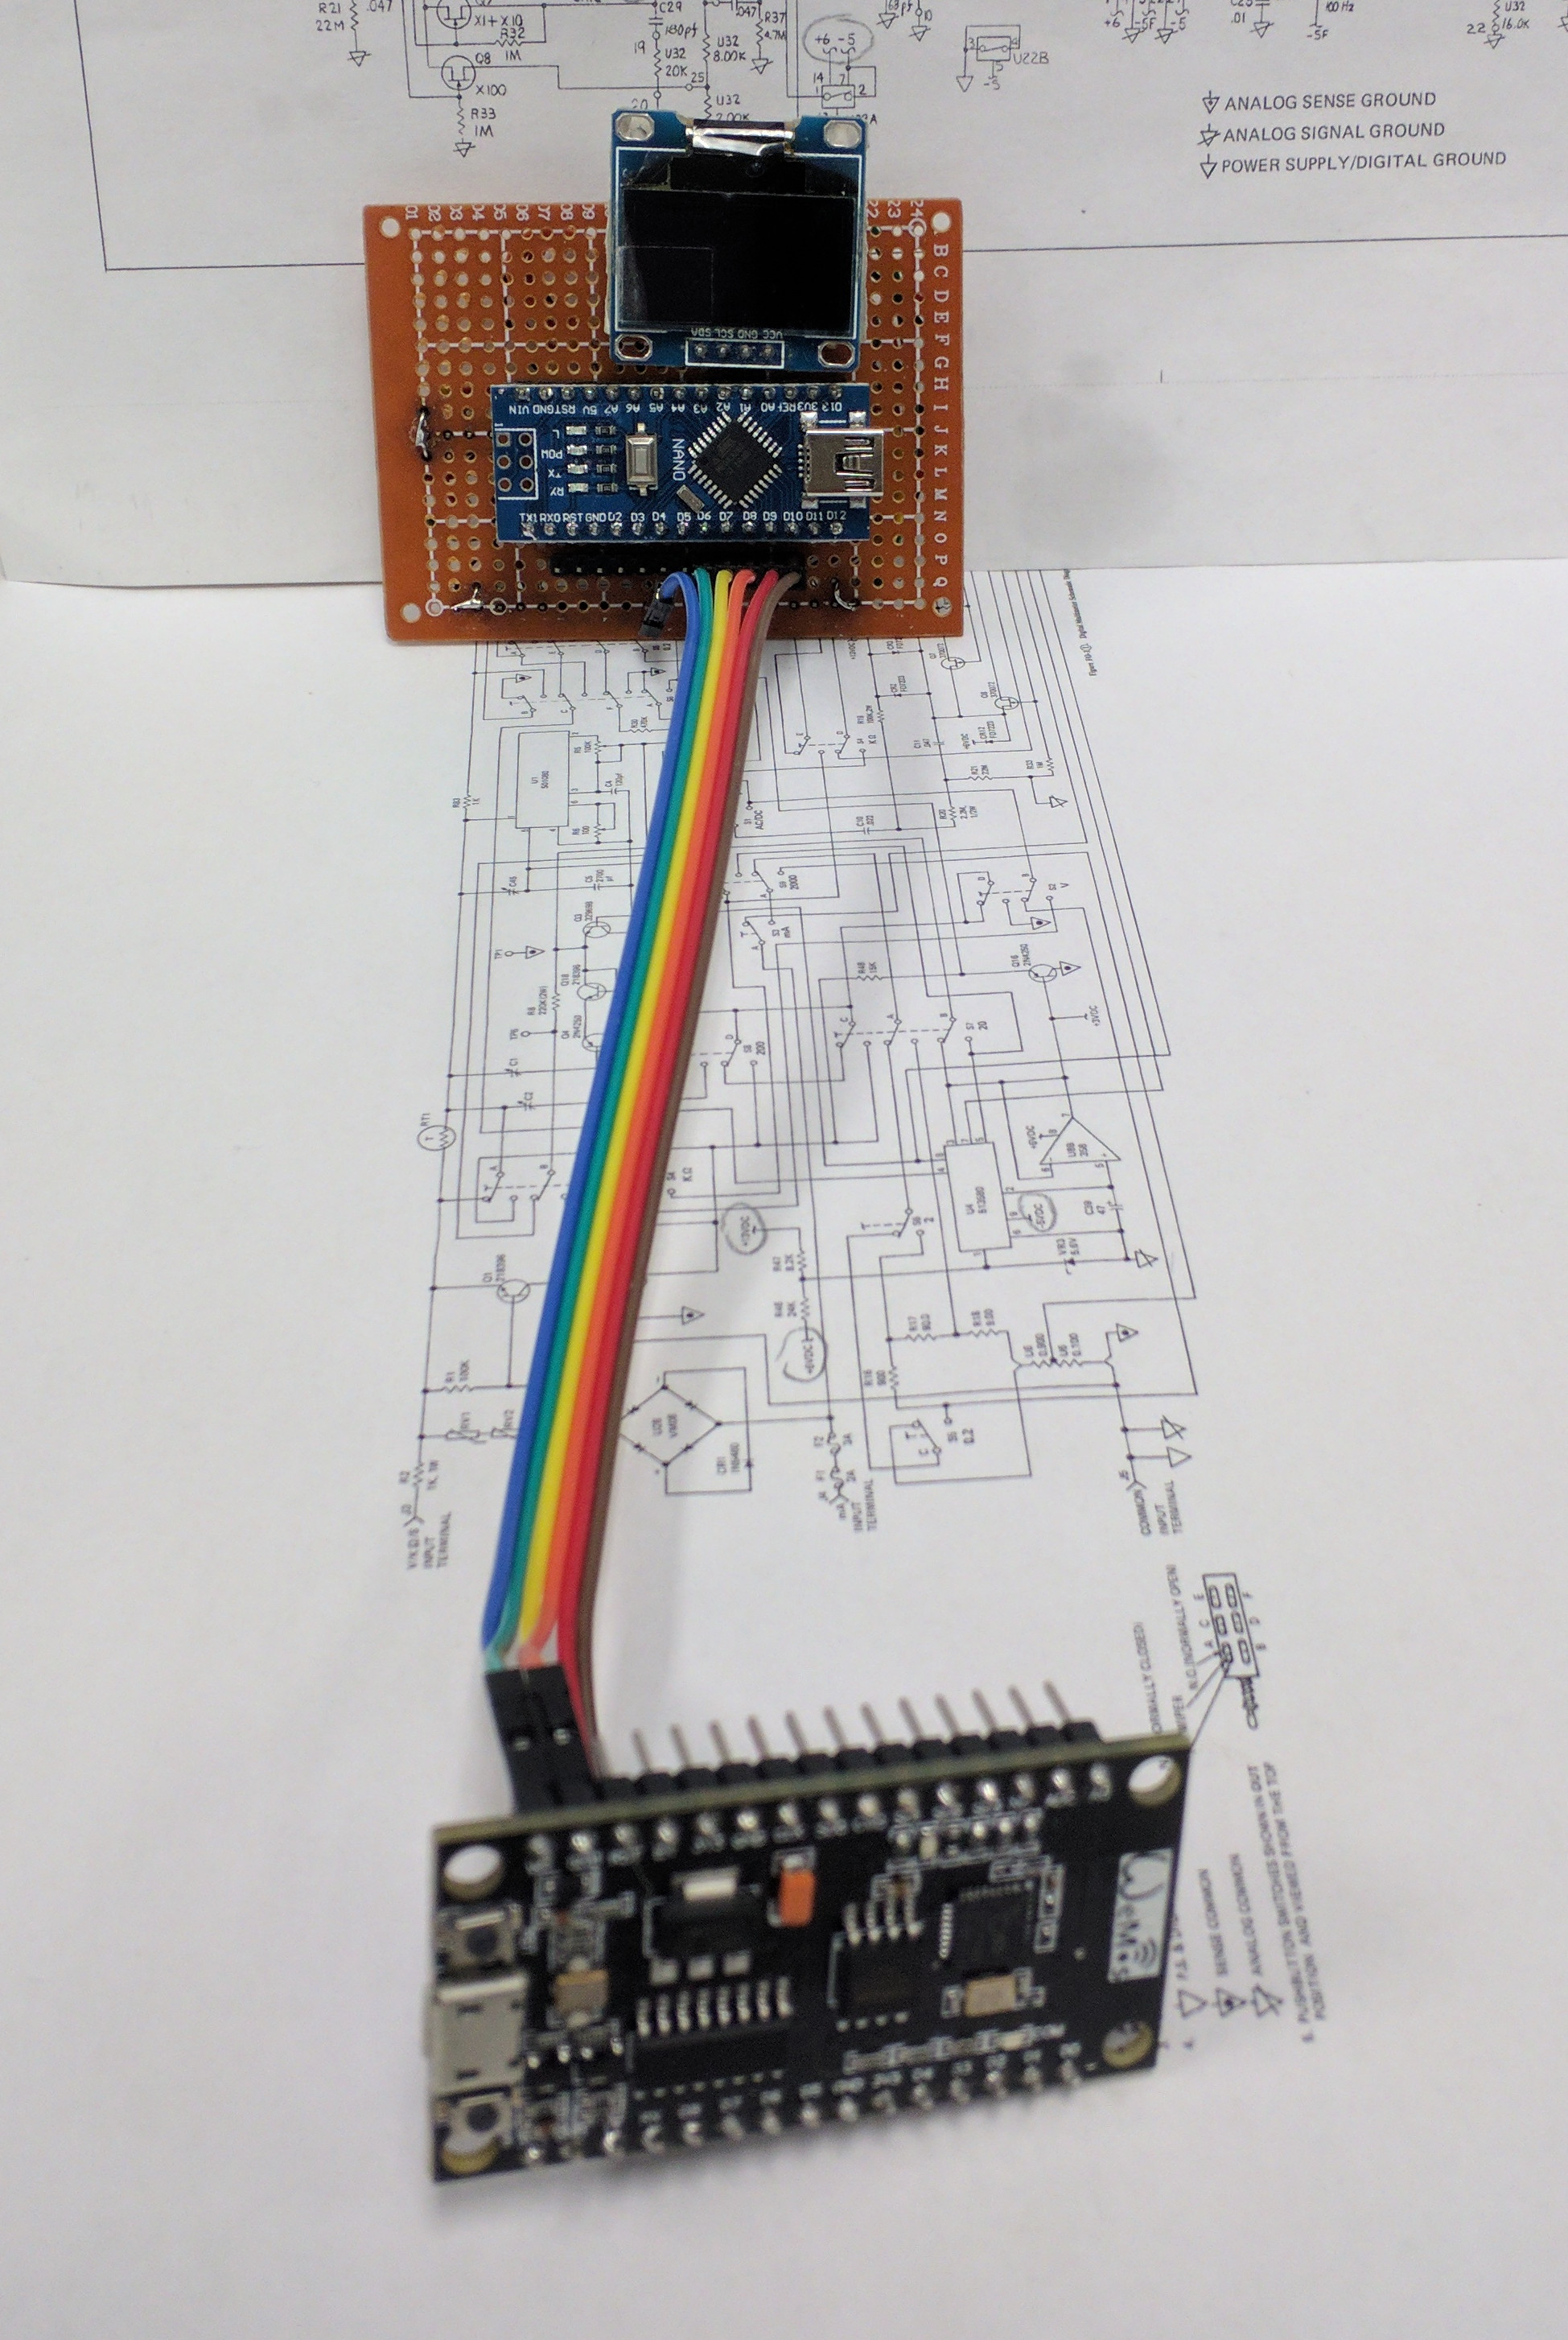
\includegraphics[width=0.40\linewidth]{figures/pic-smartshow-connected.jpg}
    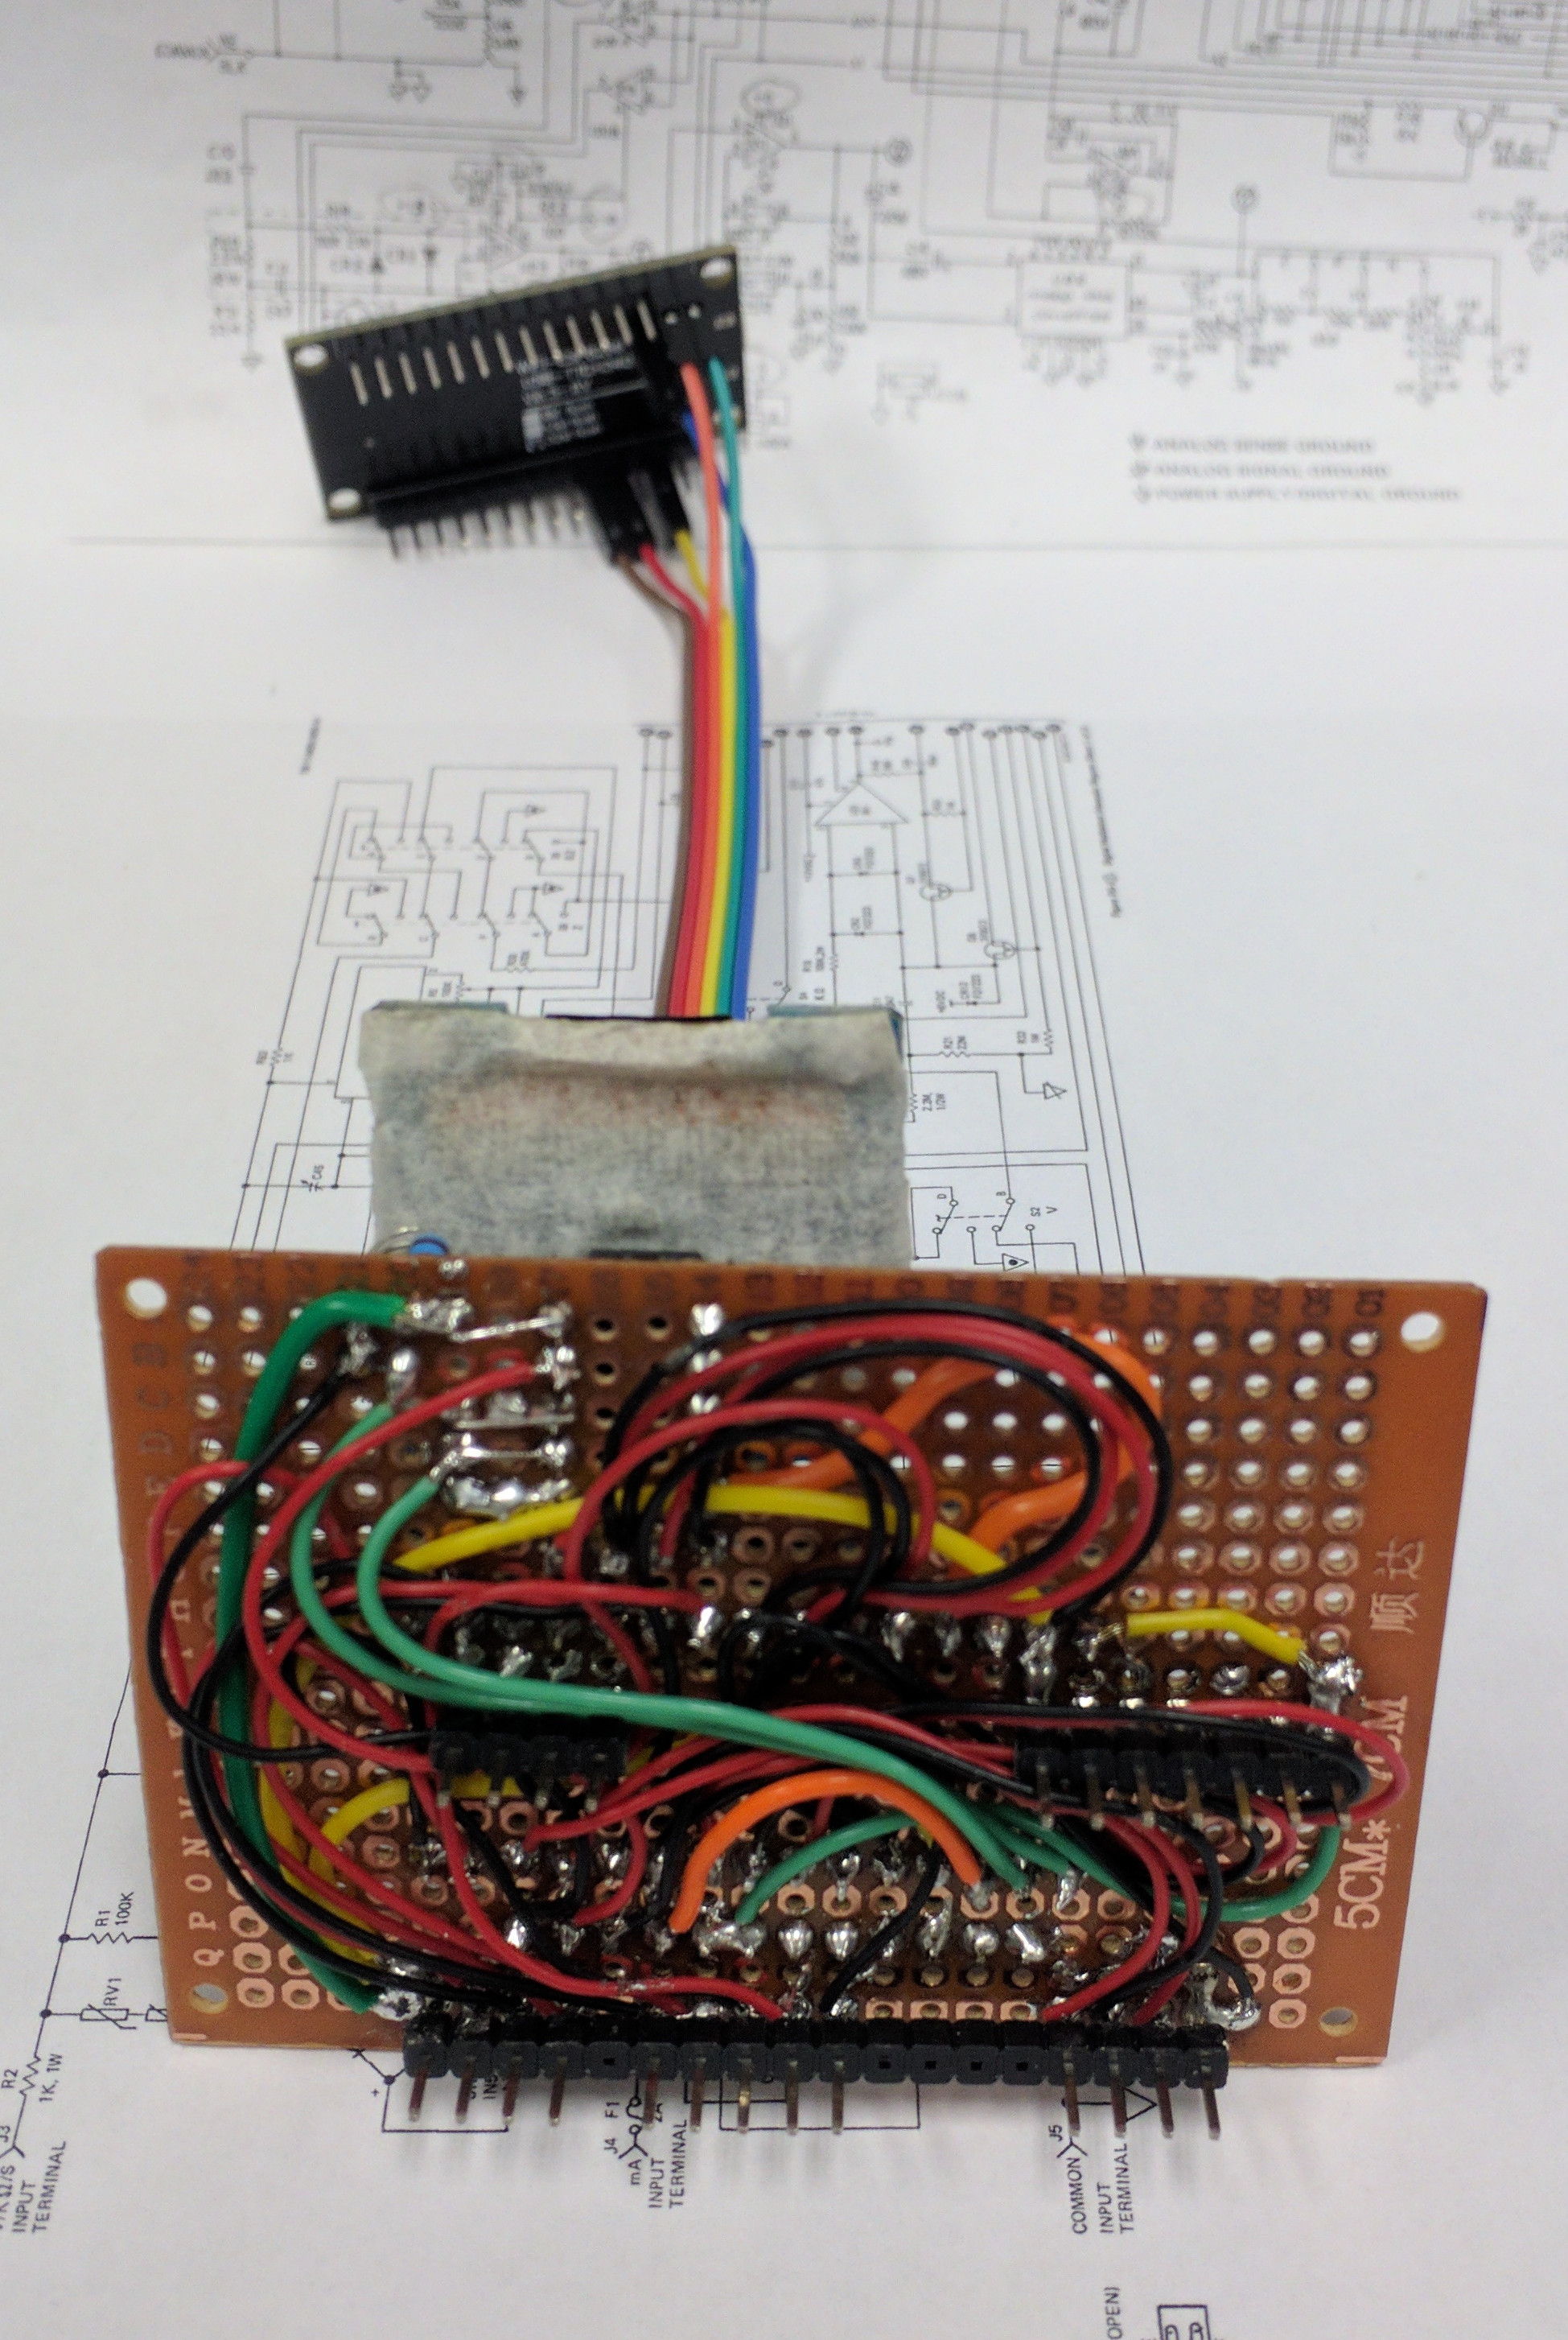
\includegraphics[width=0.40\linewidth]{figures/pic-smartshow-connected-back.jpg}
    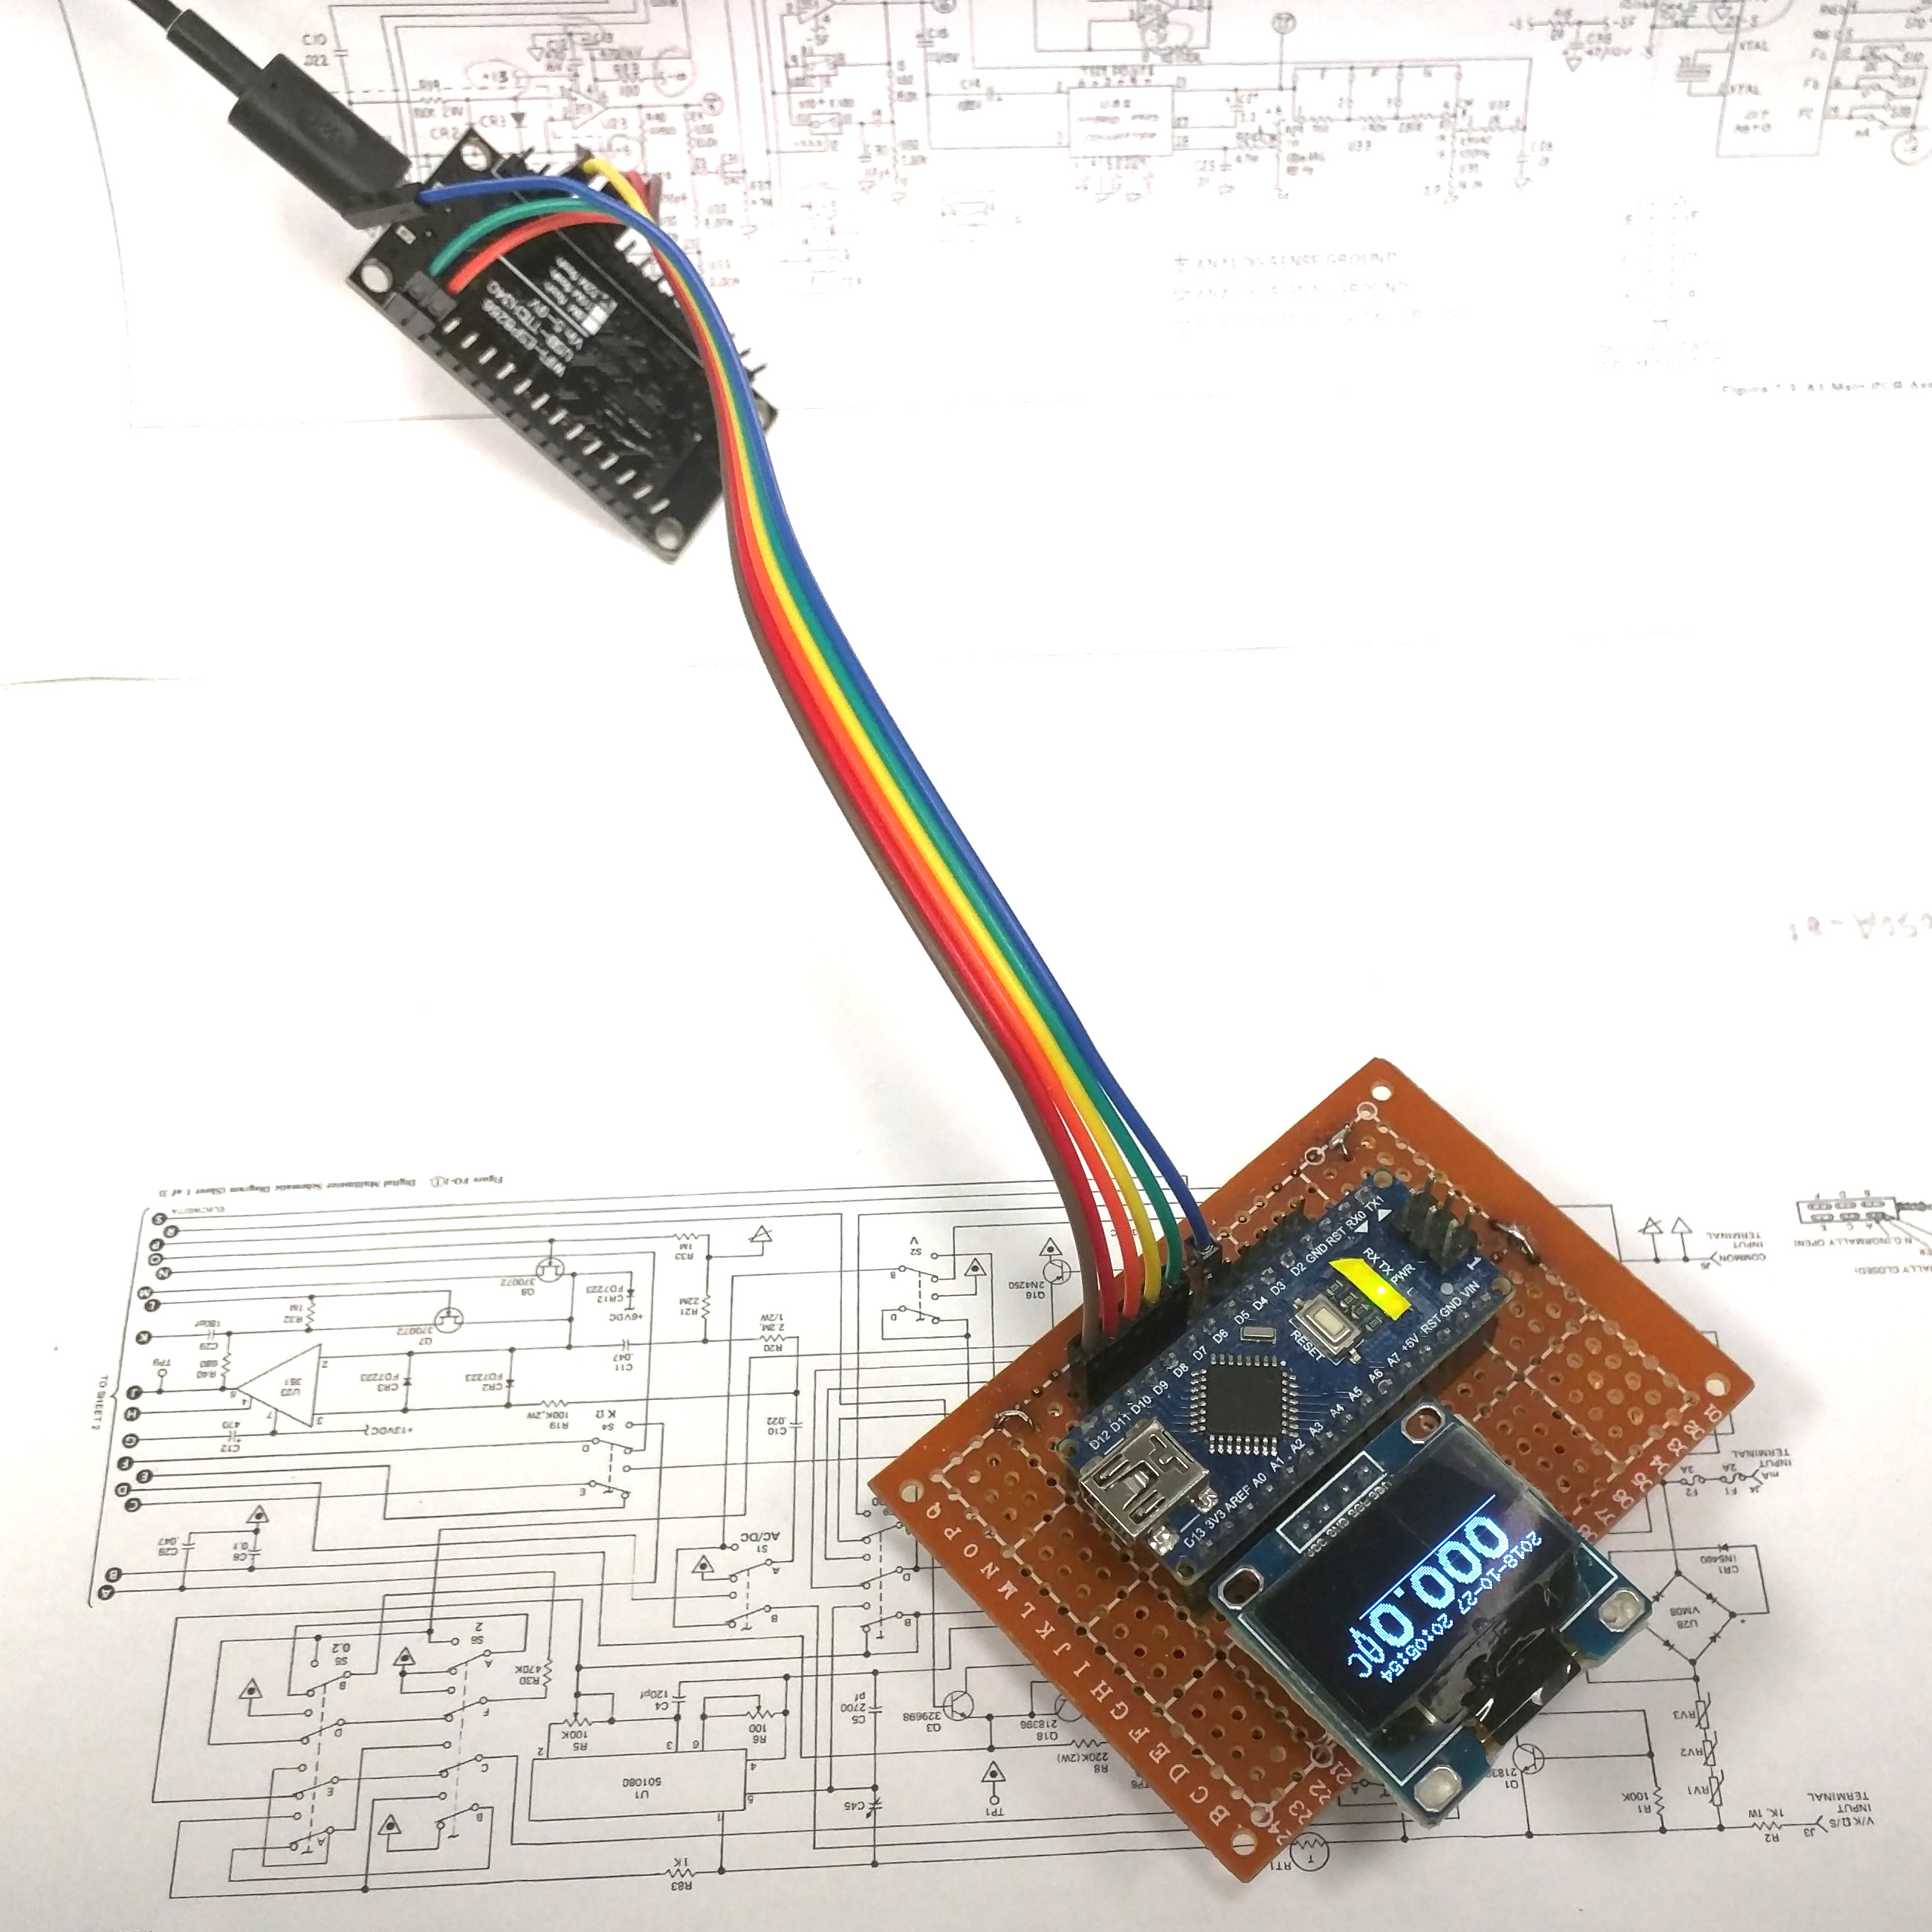
\includegraphics[width=0.60\linewidth]{figures/pic-smartshow-connected-on.jpg}
    \caption{The SmartShow main board connected to ESP module.} \label{fig:picsmmainconnesp}
\end{figure}

\subsection{Other Solutions}



\begin{figure}[h!t] \centering
    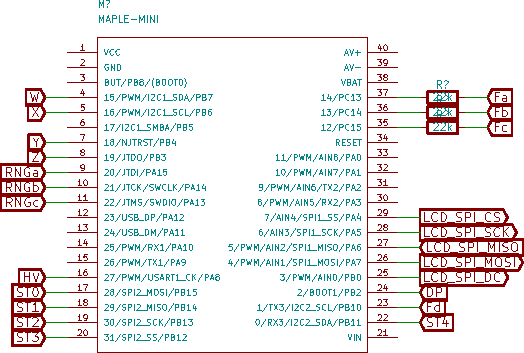
\includegraphics{figures/sch-smartshow-stm32.pdf}
    \caption{STM32(Maple-Mini).} \label{fig:smartshow-stm32}
\end{figure}



\begin{figure}[h!t] \centering
    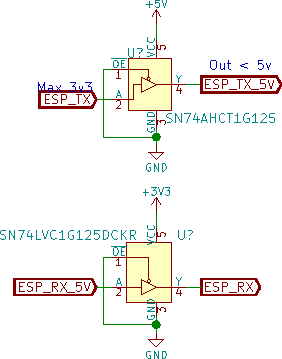
\includegraphics{figures/sch-smartshow-alt-levelshift.pdf}
    \caption{Alternative level shifting.} \label{fig:levelshiftalt}
\end{figure}










\section{Software}

The software are for both the AVR and ESP.
The ESP can also upgrade the AVR's firmware remotely.



\subsection{Configuration}

To config the hardware used in your project, you may find the file
\texttt{conf-func.h} in the directory \texttt{software/smartshow-fluke8050a/}.







\subsection{AVR}
The AVR firmware monitor the pins \texttt{ST0, ST1, ST2, ST3, ST4, ST5} etc,
and decrypt the strobe signal to value displayed in the LCD.


The strobe signal decrypt part of the source code of firmware are from the project
\href{http://vondervotteimittiss.com/belfry/?p=180}{Fluke 8050a graphic display}.


The full source project can be gotten from the repository \url{https://github.com/yhfudev/fluke8050a-screen.git}



\subsection{ESP}

For ESP, we use the project \href{https://github.com/jeelabs/esp-link.git}{esp-link}.
The pins are configured showed in the Figure \ref{fig:smartshow-confwin}.

\begin{figure}[h!t] \centering
    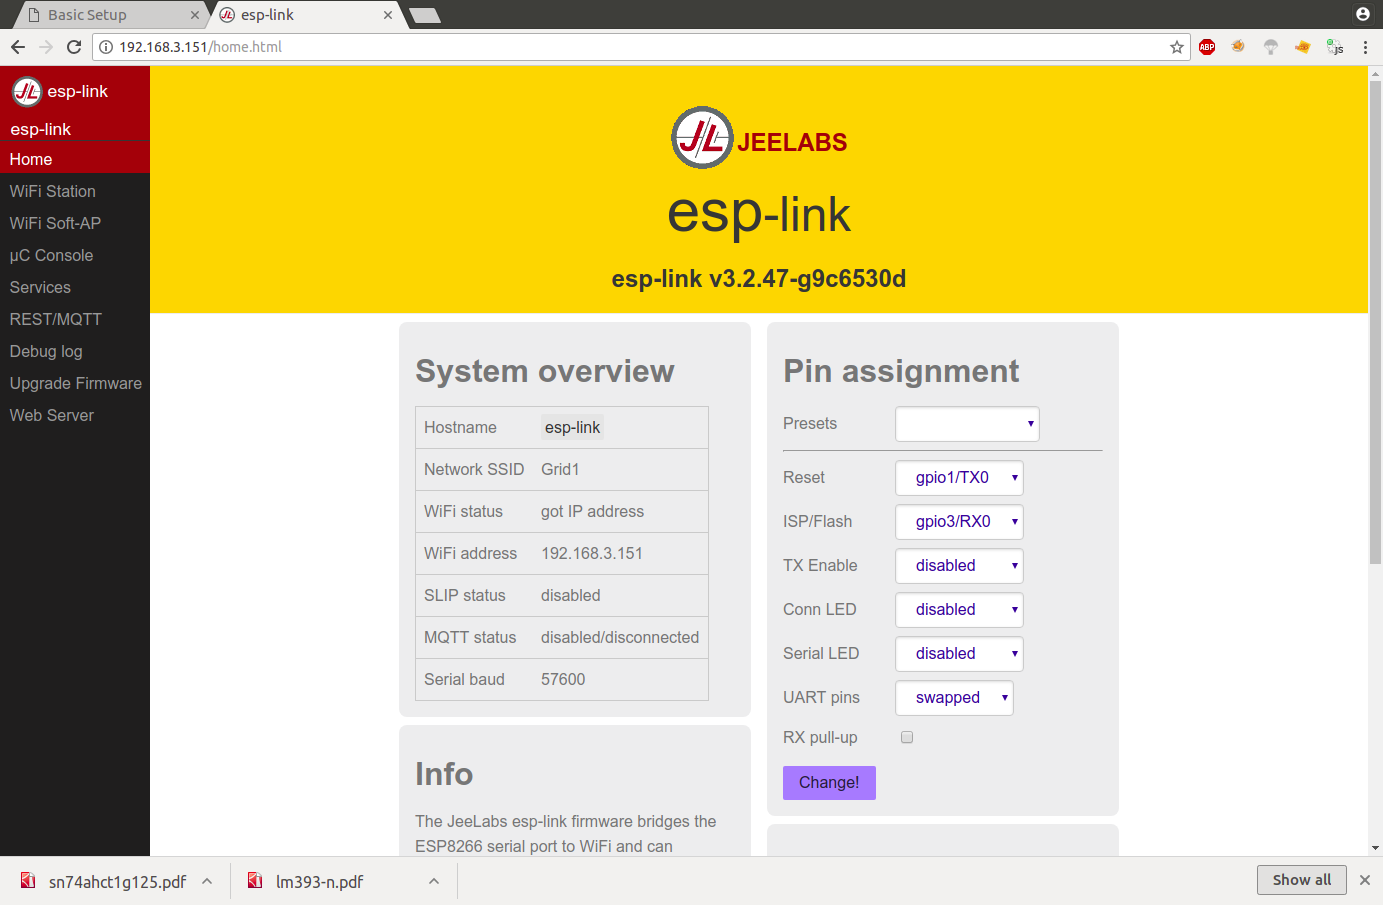
\includegraphics[width=0.8\linewidth]{figures/smartshow-confwin.png}
    \caption{Configure Pins.} \label{fig:smartshow-confwin}
\end{figure}


The data port can be accessed by either from the web UI(Figure \ref{fig:smartshow-ctrlwin}) or TCP port \texttt{23}.
\begin{figure}[h!t] \centering
    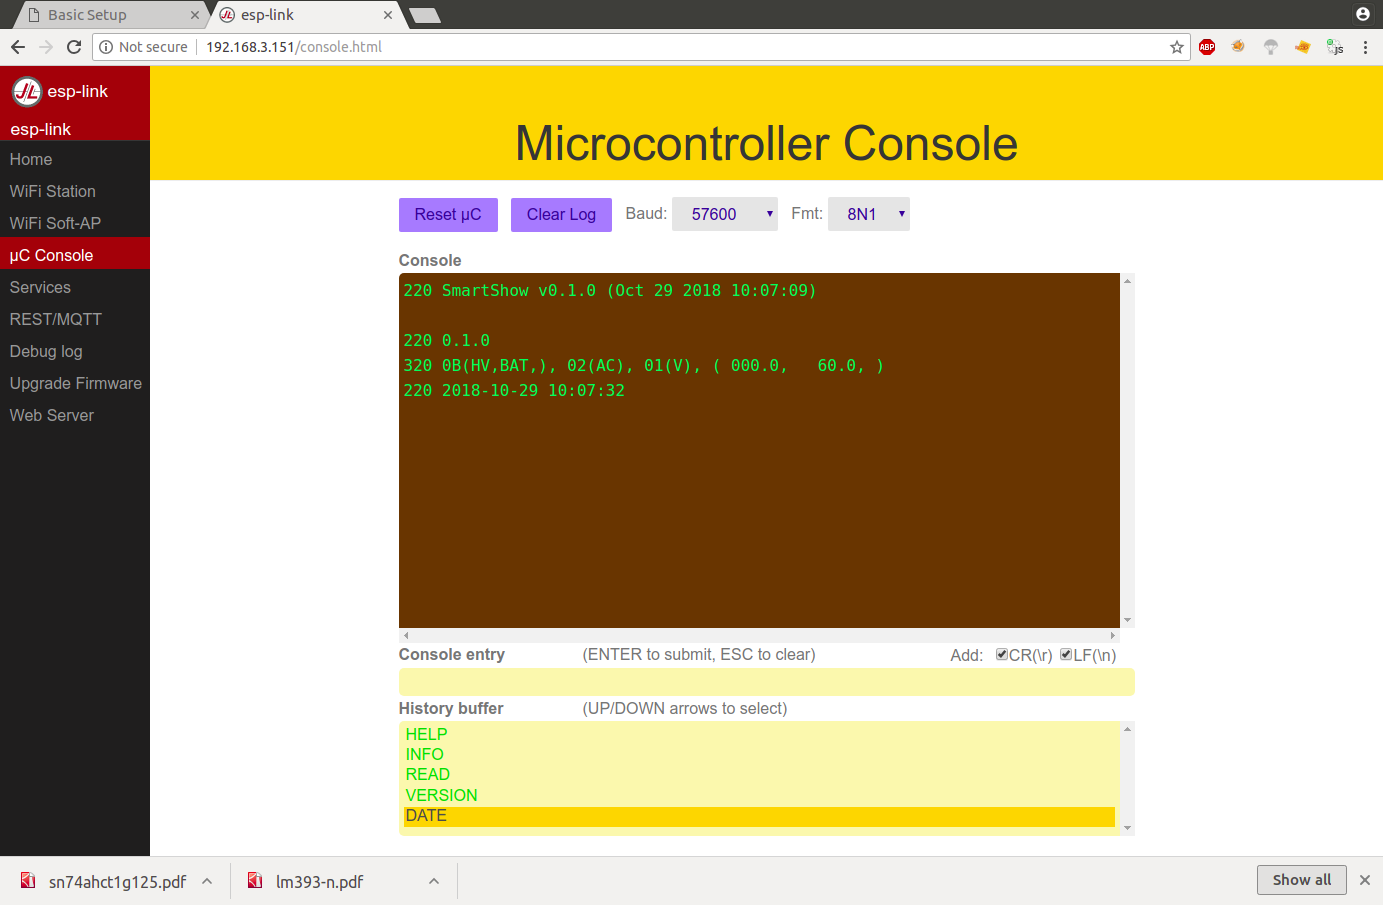
\includegraphics[width=0.8\linewidth]{figures/smartshow-ctrlwin.png}
    \caption{UART via WiFi.} \label{fig:smartshow-ctrlwin}
\end{figure}
\begin{lstlisting}[language=bash]
IP_ARDUINO=192.168.1.123
telnet ${IP_ARDUINO} 23
\end{lstlisting}




To upgrade the AVR's firmware, for example,
flash ATMega328p over Wifi:
\begin{lstlisting}[language=bash]
DN_ARDUINO="/opt/applications/arduino-1.8.5"
IP_ARDUINO=192.168.1.123
DN_HEX="/tmp/arduino_build_623246/fluke8050a-display.ino.hex"
${DN_ARDUINO}/hardware/tools/avr/bin/avrdude \
  -C${DN_ARDUINO}/hardware/tools/avr/etc/avrdude.conf \
  -v -patmega328p -carduino \
  -P  net:${IP_ARDUINO}:23 -b57600 -D -Uflash:w:${DN_HEX}:i
\end{lstlisting}





\end{document}
